\chapter{人工智能的应用}
在当今快速发展的科技时代,人工智能技术的深度融合正在深刻改变人们的生活方式、出行模式以及医疗健康服务。从智能家居的便捷生活到自动驾驶的智慧交通,再到智慧医疗的精准诊疗,这些技术的广泛应用不仅提升了生活的便利性和安全性,还为人类的健康和福祉带来了前所未有的变革。本章节将详细探讨这些领域的最新进展及其对现代社会的深远影响,揭示智能科技如何为人们的生活带来更加智能化、高效化和个性化的体验。

\section{智慧生活}

智能家居、智能助理、智能娱乐与个性化推荐在日常生活中广泛应用。人工智能技术和互联网技术\footnote{物联网技术(Internet of Things,IoT)的核心理念是通过互联网将各种智能设备互联互通,实现远程控制、数据交换和智能化管理。}的结合实现设备的互联互通与智能管理,提升生活的便利性、安全性和娱乐体验。智能家居通过灯光、温控、安防设备等优化居住环境;智能助理利用自然语言处理实现便捷交互;智能娱乐系统通过分析用户行为提供个性化内容推荐。这些技术的集成推动生活方式向更加智能化和自动化的方向发展,显著提升用户的整体生活质量。

\subsection{智能家居}

智能家居系统逐渐渗透到日常生活的各个方面,不仅能够独立运行各类设备,还能通过网络与其他设备协作,提升生活环境的智能化水平。利用人工智能技术,家庭自动化系统进一步实现了环境的自动调节和智能管理,显著提高了生活的便利性和舒适度。以下将详细探讨智能灯光、智能温控和智能安防设备如何通过人工智能技术和物联网技术实现互联互通,打造智能家居环境。

\begin{figure}[ht]
  \centering
  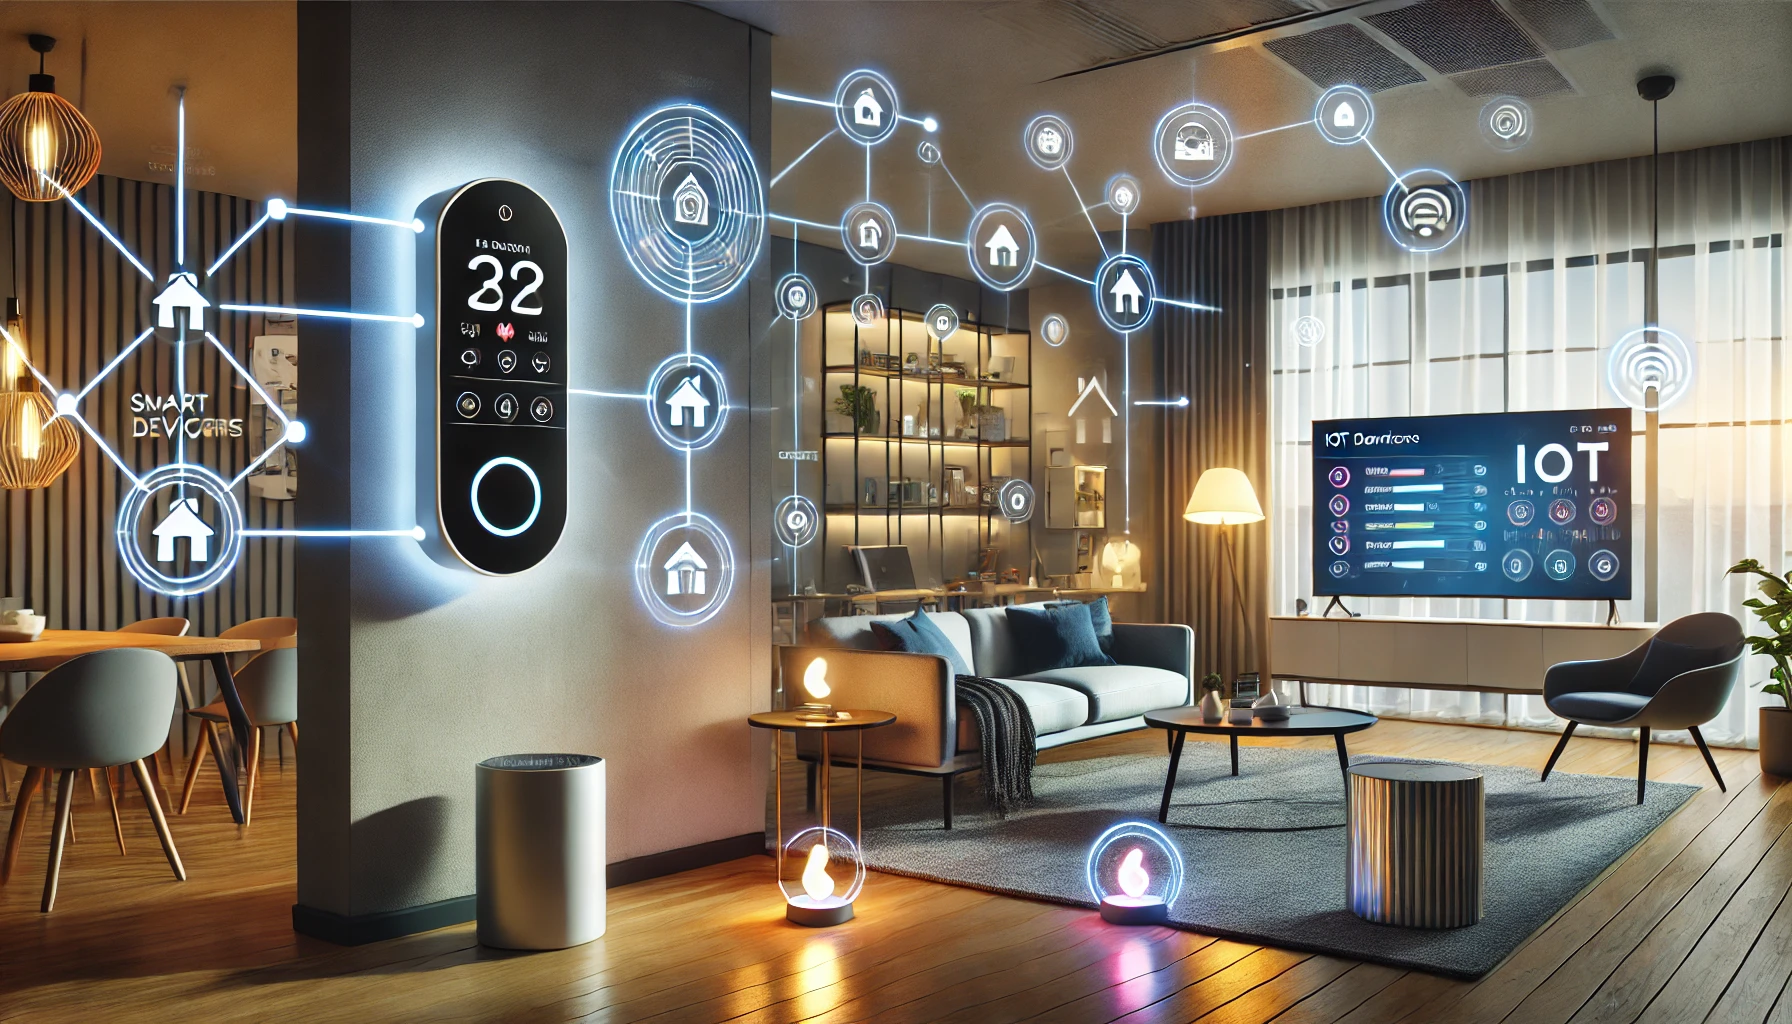
\includegraphics[width=\linewidth]{image/4/智能家居.png}
  \caption{智能家居理念图(图片由AI生成)}
  \label{fig:智能家居}
\end{figure}

\subsubsection{1.家庭自动化系统的工作原理}

家庭自动化系统的核心在于物联网技术与人工智能的结合。通过传感器、智能设备和云计算平台,家庭环境中的各类设备能够实时采集和处理环境数据,并通过人工智能算法进行智能分析与决策,自动调整设备的工作状态,完成各类任务。例如,智能温控系统根据室内外温差自动调节空调温度,智能照明系统根据光线强度自动调节灯光亮度,智能安防系统自动监控家庭安全,避免不必要的麻烦和安全隐患。

以某国产家居为例,其全屋智能系统涵盖了智能灯光、智能家电、安防系统和环境控制等多个领域。用户可以通过智能门锁实现回家时的自动化场景,门锁开启后,联动智能灯光和窗帘自动调整,营造温馨的回家氛围。同时,智能温控设备如空调伴侣,能够根据室内外温度变化和用户习惯自动调节空调运行状态,实现节能和舒适兼顾。在安防方面,门窗磁传感器、烟雾报警器等设备能够实时监测家庭安全,一旦发生异常情况,及时向用户发送警报信息,全方位保障家庭安全。

家庭自动化系统依赖物联网和人工智能技术,为用户提供便捷、安全的生活环境。其运作环节包括数据收集、传输和处理,以及人工智能的决策优化。智能传感器的信息获取、数据处理和决策过程是家庭自动化系统的核心,深入探讨这些环节可以更好地理解该系统的功能与效果。

\begin{enumerate}
    \item \textbf{智能传感器获取信息}:家庭自动化系统依赖多种传感器实时感知环境信息,如温度传感器、湿度传感器、光照传感器、运动传感器和声学传感器。这些传感器不断向系统发送数据,系统根据这些数据判断何时执行自动化操作。
    \item \textbf{数据传输与处理}:传感器采集的数据通过无线网络(如Wi-Fi、Zigbee、Bluetooth)传输至中央控制系统,或直接上传到云端平台进行处理。通过强大的数据处理能力,人工智能算法能够从大数据中提取有价值的信息,实现对设备的精准控制和预测性维护。
    \item \textbf{人工智能决策与优化}:基于机器学习和深度学习算法,家庭自动化系统能够分析历史数据,识别用户行为模式。例如,通过分析过去几周的温度变化,系统可以预测未来的温度变化,并提前调节温控系统,确保室内始终保持舒适温度。人工智能还能够根据用户偏好动态调整操作策略,提供更加个性化的服务。
\end{enumerate}

接下来将详细探讨智能家居中的各个关键组成部分,包括智能灯光、智能温控和智能安防系统等。

\subsubsection{2.智能灯光}

智能灯光系统是智能家居中的基础组成部分之一,通过物联网技术实现远程控制、自动调节和数据分析等功能。智能灯具内嵌传感器,能够实时感知环境变化,并根据预设规则进行调整。具体工作原理如下:

智能灯光通过嵌入式传感器和无线通信技术(如Wi-Fi、Zigbee、Bluetooth等)与物联网系统连接。通过手机APP或语音助手发出指令,智能灯泡接收到命令后,自动调整光亮度、色温或颜色。此外,智能灯具还可通过环境传感器感知到周围的光线变化,自动调节亮度以节省电能。例如,当感应到室内有足够自然光时,智能灯具会自动调暗,反之则调亮。

智能照明系统通过调节亮度和颜色,满足不同场景需求,如家庭中的定时开关和情境模式(如早晨唤醒或夜晚阅读模式),或在商业场所中根据人流量自动调整光线强度,提升工作效率并节能。此外,智能灯光可与其他智能设备互联互通,如与温控、安防系统及语音助手协作,自动感应环境变化,增强用户体验并实现能源节约。

\subsubsection{3.智能温控}

智能温控系统(如智能空调、智能暖气和智能恒温器)是物联网在家庭和商业环境中应用的重要领域之一。通过连接至物联网平台,智能温控设备能够自动调节室内温度,确保舒适环境的同时最大程度地节省能源。

智能温控系统由传感器、控制器、执行器和联网模块组成。传感器检测环境温度变化后,信息通过物联网连接传递给中央控制系统,控制系统基于设定参数决定加热或降温,最终通过执行器调节温控设备(如空调、暖气)的工作状态。此外,智能温控系统能够学习用户的生活习惯,并根据这些习惯进行自动调整。例如,在用户习惯的回家时间前,智能温控系统会提前调节室内温度,确保回家时室内温暖或凉爽。

智能温控系统广泛应用于家庭和商业场所,通过自动调节温度来提升舒适度并节能。在家庭中,系统根据用户的作息规律调整温度,如睡觉时自动调低室温以节省能源,早晨起床时恢复舒适温度,且用户可远程通过智能手机进行控制,确保回家时温度宜人。在商业环境中,智能温控根据员工人数和活动量自动调整温度,无人时进入节能模式,大量员工进入时恢复设定舒适温度。此外,智能温控系统与其他智能设备互联互通,例如与智能灯光系统联动,自动感应房间内是否有人,并根据情况同时开启或关闭温控与灯光,或通过智能家居平台优化室内舒适度,进一步提升能源效率与用户体验。

\subsubsection{4.智能安防}

智能安防系统通过物联网技术实现对家庭、办公室等环境的全天候安全监控。这些系统结合多种智能设备,如智能摄像头、门禁系统、门窗传感器和运动探测器,能够实时监控并响应潜在的安全威胁。

智能安防系统集成摄像头、传感器和报警设备,使用无线通信技术(如Wi-Fi、Zigbee、LoRa等)将数据传输到云平台或智能终端。当传感器检测到异常事件(如门窗被打开、运动探测到异常等)时,立即通过网络将警报信息传输给用户或安防中心,启动报警系统,甚至自动联系当地执法机构进行响应。

智能安防系统在家庭和商业场所中应用广泛,提升了安全性和便利性。在家庭中,智能门锁和监控摄像头帮助用户远程查看门外情况并决定是否允许访客进入,同时与安防系统结合,在发生盗窃或非法入侵时自动触发报警并通知房主或安保人员。
商业场所则通过集成传感器和摄像头实时监控门窗和敏感区域,及时检测未授权人员入侵并报警,系统还可通过面部识别提供个性化服务。

智能安防系统与其他智能设备互联互通,进一步增强安全性,例如与智能温控系统联动,入侵发生时自动关闭空调或暖气,减少异常活动的迹象;与智能灯光系统联动,在检测到潜在威胁时自动开启灯光,制造有人在家的假象,从而威慑不法分子。

\subsubsection{5.人工智能驱动的家庭自动化系统的未来发展}

未来,人工智能技术将在家庭自动化系统中发挥更加重要的作用。随着5G、边缘计算以及更强大的人工智能算法的发展,家庭自动化系统将实现更高效、更智能的功能。例如,人工智能将能够更好地预测用户需求,动态调整家庭环境参数,并与更多智能设备无缝连接。未来的智能家居不仅能够理解用户的偏好和行为模式,还能够通过更加精细化的控制实现高度个性化的体验。

此外,随着智能家居生态系统的逐步完善,家庭自动化系统将更加注重安全性、隐私保护与数据共享的问题。人工智能技术将确保用户数据的安全,同时实现设备之间的高效协作,为家庭提供更加智能、安全、环保的生活方式。

\subsubsection{6.小结}

智能家居通过物联网和人工智能技术实现高度的互联互通,极大提升了生活的便利性和舒适度。智能灯光、智能温控和智能安防设备在物联网和人工智能的支持下,能够根据环境变化、用户需求和设备状态进行智能调节与协作,为智能家居环境提供全面的支持。随着技术的不断进步,未来的家庭自动化系统将更加智能化,实现更高层次的自动化和自适应能力,全面提升用户体验。

\subsection{智能助理}

智能助理在现代智能家居和智能办公场景中占据着重要地位。通过语音识别和自然语言处理等技术,智能助理能够实现与用户的自然交流,提供便捷、高效的服务。2025年爆火的DeepSeek就属于一款智能助理。它改变了人们在偌大的信息世界获取有效资源的方式,也改变了人们解决问题的方式,大大降低了技术门槛。以下内容将详细介绍语音识别技术在智能助理中的应用,以及自然语言处理与对话系统如何实现人机自然交互。

\subsubsection{1.语音识别技术}

语音识别技术是智能语音助理的核心组成部分,旨在将用户的语音指令转换为可理解的文本或指令,通过第三章所述的声音采样、量化和信号处理等步骤,实现信息的获取和识别。

\begin{figure}[ht]
  \centering
  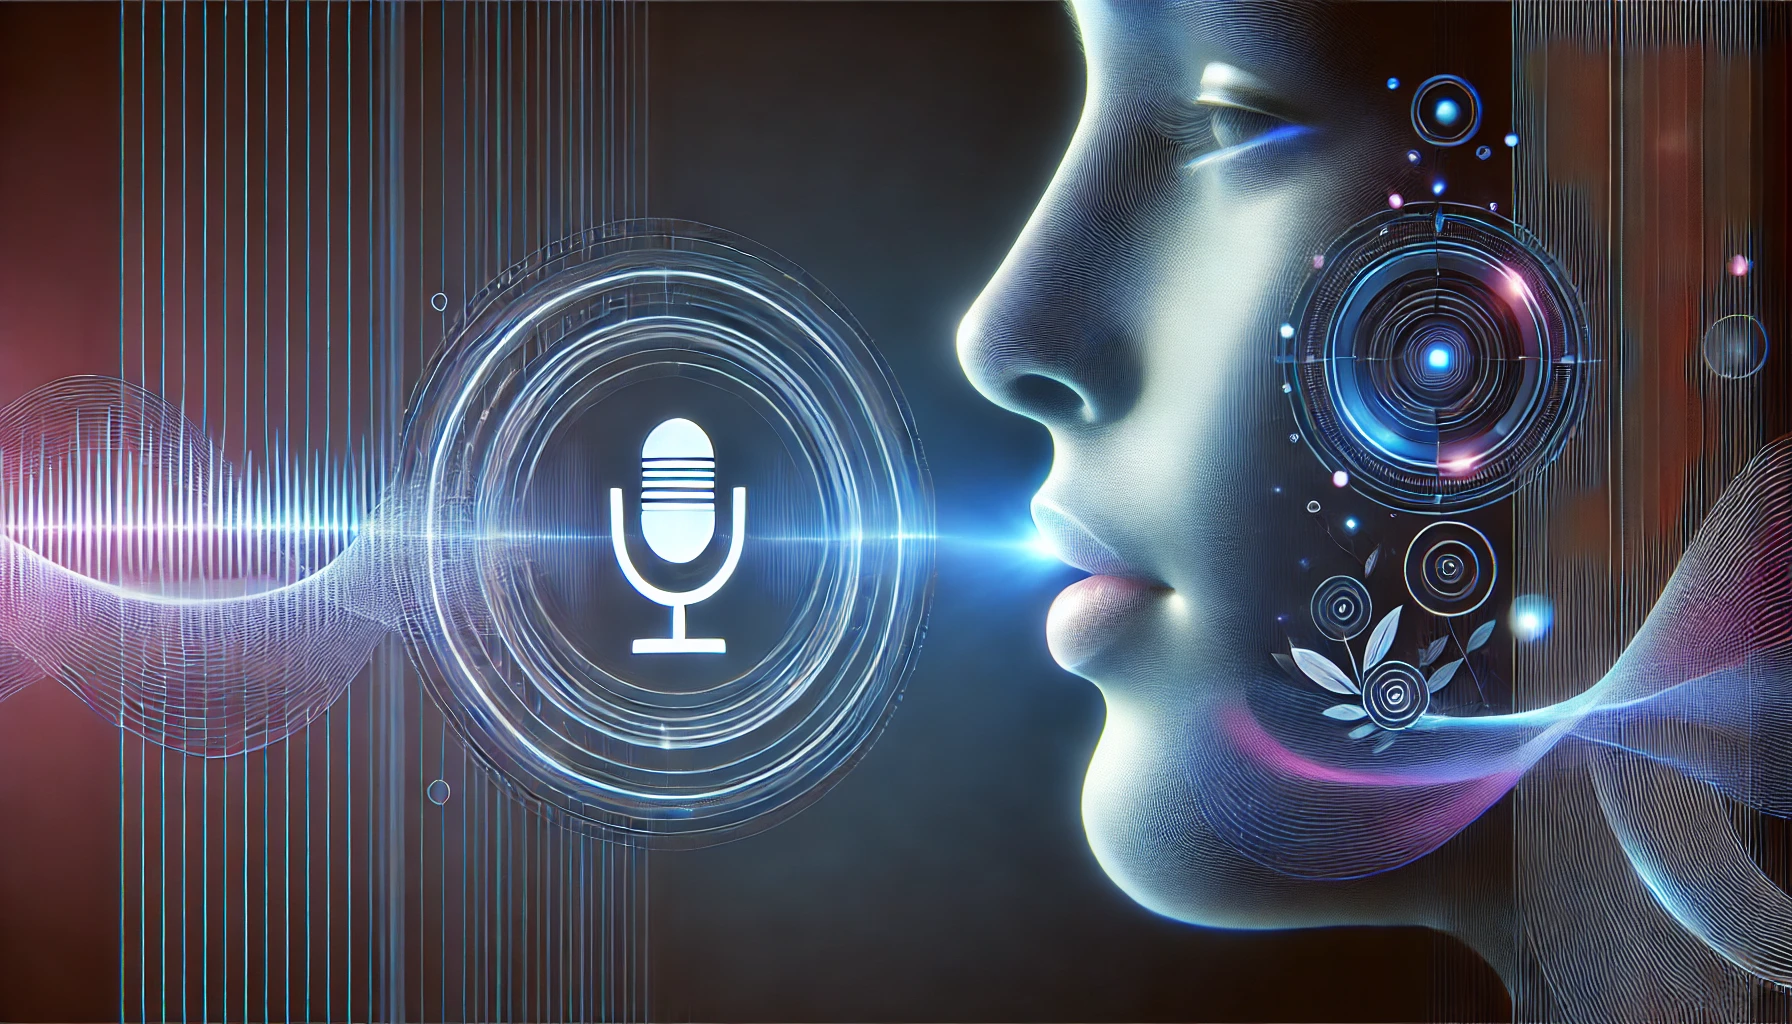
\includegraphics[width=\linewidth]{image/4/智能语音助手.png}
  \caption{智能语音助手(图片由AI生成)}
  \label{fig:智能语音助手}
\end{figure}

% 语音识别技术主要包括以下几个步骤:

% \begin{enumerate}
%     \item \textbf{声音采集}:通过麦克风设备采集用户的语音信号,并将其转化为数字信号\footnote{数字信号是用离散的数值或符号表示信息的信号,与连续信号相对,常用于电子通信和数据处理。}。这一过程涉及声音的捕捉和初步的信号处理,以确保后续步骤的准确性。
%     \item \textbf{信号处理}:对采集到的语音信号进行预处理,包括噪声消除、回声抑制和信号增强等,以提高语音信号的质量和识别的准确性。
%     \item \textbf{特征提取}:从预处理后的语音信号中提取关键特征,如梅尔频率倒谱系数(MFCC)\footnote{梅尔频率倒谱系数(MFCC)是一种用于语音和音频信号处理的特征提取方法,它通过将音频信号转换为梅尔频率尺度上的倒谱系数,帮助捕捉人类听觉感知的特性,从而有效地表示声音的频谱信息。}、声学特征等。这些特征用于描述语音的基本属性,为后续的模式匹配提供依据。
%     \item \textbf{模式匹配}:将提取的语音特征与预先训练的声学模型进行比对,识别出对应的文字或指令。声学模型通常基于深度神经网络(DNN)、卷积神经网络(CNN)或循环神经网络(RNN)等先进的机器学习算法。
%     \item \textbf{后处理}:对识别结果进行语法校正和上下文理解,生成最终的文本输出或执行指令。这一过程包括语言模型的应用,以确保输出内容的连贯性和准确性。
% \end{enumerate}

目前,有一些人工智能助手支持多语言识别,能够理解复杂的语音指令,提供精准的搜索结果和智能家居控制。集成了强大的搜索引擎和信息处理能力,提升了用户的交互体验。提供语音控制、信息查询、任务管理等功能,提升用户体验。还可以与手机生态系统的深度整合,实现无缝的设备控制和信息获取。

还有的助手,不仅能够响应用户的语音指令,还能在多轮对话中理解用户的意图。例如,用户可以对助手说“今天心情好不好?”,助手会以幽默的方式回应,随后用户可以连续发出不同的指令,如“打开书房灯”、“亮度调暗一点”、“放一首《燕归巢》”,助手都能一一响应。此外,助手还能在用户需要时提供信息查询服务,比如询问时间,助手会准确告知当前时间。

用户还可以对助手使用简单的语音指令控制智能家居设备,如“打开音乐并导航回家”,助手便能协助完成这一系列动作。在影音娱乐方面,用户只需呼叫助手,就能帮助调高音量、播放电影、打开窗帘、关闭空调,打造沉浸式观影体验。助手还能在运动健康领域提供帮助,比如用户说“开始跑步”,手表就会开始记录跑步数据,并进行实时播报。


虽然语音识别技术已经非常成熟,但是仍面临诸多挑战,包括不同口音的识别、背景噪声的干扰、语音的连贯性和自然性等。近年来,随着深度学习和神经网络技术的发展,语音识别的准确性和鲁棒性\footnote{鲁棒性是指系统在面对不确定性、变化或干扰时仍能保持良好性能和稳定性的能力。}得到了显著提升。特别是基于卷积神经网络和循环神经网络的模型,能够更好地捕捉语音信号中的时序和空间特征,显著提高了识别效果。

此外,端到端的语音识别模型(如Transformer架构\footnote{Transformer架构是一种深度学习模型,主要用于自然语言处理,它通过自注意力机制和并行处理能力,显著提高了序列数据的处理效率和效果。})进一步简化了传统语音识别流程,提高了模型的训练效率和识别准确性。通过大规模的数据训练,这些模型能够适应各种复杂的语音环境和用户需求。

\subsubsection{2.自然语言处理与对话系统}

自然语言处理与对话系统是实现智能助理与用户自然交互的关键技术。通过理解和生成自然语言,智能助理能够准确理解用户意图,并提供相应的回应和服务。
自然语言处理技术包括自然语言理解\footnote{自然语言理解(Natural Language Understanding,NLU):旨在解析用户的语音或文本输入,理解其中的意图和实体。主要包括语义分析、句法分析、情感分析等。NLU技术通过识别用户意图(Intent Recognition)和提取关键实体(Entity Extraction),实现对用户需求的准确把握。}和自然语言生成\footnote{自然语言生成(Natural Language Generation,NLG):根据理解到的意图和上下文信息,生成符合语法和语境的自然语言回应。NLG技术通过构建语言模型,确保生成的回应既准确又自然,提升用户的交互体验。}两个主要部分。

对话系统通常由多个关键部分组成。首先,意图识别通过自然语言理解技术识别用户的意图,例如查询天气、播放音乐、设置闹钟等。这一步骤是对用户需求进行分类和理解的关键。接下来,实体提取从用户的输入中提取关键信息,如日期、地点、时间等。这些实体信息用于进一步完善用户请求的细节,确保回应的准确性。

在理解用户意图和提取相关实体信息之后,对话管理根据用户的意图和上下文信息,制定对话策略,决定下一步的响应或操作。对话管理系统通过维护对话状态和上下文,实现多轮对话的连贯性和逻辑性。最后,响应生成通过自然语言生成技术生成自然、连贯的回应,提升用户的交互体验。响应生成不仅关注语法正确性,还注重回应的内容和情感表达,使对话更加人性化。

一个完整的对话系统通过意图识别、实体提取、对话管理和响应生成等多个部分的协同工作,能够有效理解并响应用户的需求,提供流畅且智能的交互体验。

智能助理通过对话系统实现与用户的自然交互,主要体现在多个方面。它能够处理连续的、多轮的对话,保持上下文一致性和连贯性。例如,用户询问“明天的天气如何?”,智能助理不仅回答天气情况,还能继续回答相关的出行建议。

此外,智能助理通过情感分析技术,能够识别用户的情感状态,调整回应的语气和内容。例如,当用户表达不满时,智能助理会以更加温和的语气回应,以提升用户的满意度。

通过学习用户的偏好和习惯,智能助理还能够提供个性化的服务和建议,例如根据用户的日常作息,提前提醒重要事项或安排日程。

比如,由深度求索公司研发的DeepSeek具备先进的自然语言理解和生成能力,能够进行流畅的对话并提供准确的信息。DeepSeek通过不断学习和适应用户的交流方式,提供个性化的回答和建议。例如,用户可以询问“如何制作意大利面?”,DeepSeek不仅会提供详细的烹饪步骤,还能根据用户的反馈进行调整,比如“少油少盐的版本”。DeepSeek 正成为连接人类与数字世界的“智能桥梁”。无论是解决“今晚吃什么”的生活选择,还是处理“商业合同风险评估”的专业需求,其自然流畅的交互体验让技术真正“隐身”,只留下高效与便捷。

DeepSeek支持超长对话,并能通过用户习惯学习优化回答风格。例如,若用户常要求“用比喻解释复杂概念”,AI 会逐渐在回答中增加类比。其次,各种语言无缝切换,可实时翻译并生成100+种语言内容,支持方言理解(如粤语、四川话),甚至能识别网络流行语并合理运用。通过微表情符号、语气词判断用户情绪,动态调整回复策略。如检测到用户输入“这题太难了[哭泣的表情])”,AI 会自动切换鼓励性话术并提供分步指导。

% \begin{figure}[htb]
% 	\centering
% 	
\includegraphics[width=\linewidth]{image/0/deepseek.png}
% 	\caption{DeepSeek交互界面}
% 	\label{DeepSeek图片}
% \end{figure}

DeepSeek拥有三种不同的模式,基础模型、深度思考模型、联网搜索。它们有各自的使用场景,共同构建了覆盖全场景的智能服务体系。
其中通用模型适用于大多数日常任务。它的特点是超快速的响应速度和广泛的适用性,能够帮助用户高效完成各种简单的任务。无论是生成创意文案、撰写社交媒体帖子,还是总结知识点、整理会议纪要,基础模型都能以极高的效率提供高质量的结果。对于普通用户来说,这一模式就像是一个随叫随到的智能助手,能够在日常生活中提供即时的帮助和支持。基础模型的存在让用户无需担心繁琐的操作流程,只需简单输入需求即可获得结果,真正实现了人工智能在日常生活中的无缝渗透。
而深度思考模型是一种推理模型,专注于解决需要高度逻辑分析和推理的任务。相比基础模型,深度思考模型在推理能力、逻辑分析和决策支持方面表现更为卓越。它不仅能够理解复杂的上下文信息,还能输出结构化的分析报告,为用户提供深入的洞察。通过深度思考模型,用户可以从表面现象深入挖掘本质问题,突破复杂问题的边界,实现更高层次的智能化应用。
联网搜索模式将人工智能与互联网海量信息相结合,为用户提供实时的数据支持。联网搜索模式能够精准捕捉市场动态、学术前沿以及社会热点等实时数据,帮助用户掌握最新趋势。

DeepSeek 的三种模式并非孤立存在,而是相辅相成,共同构成了一个完整的智能服务体系。用户可以从基础模型入手,体验人工智能在日常生活中的便捷性;当遇到复杂问题时,切换到深度思考模型,借助强大的推理能力和分析工具解决问题;最终通过联网搜索模式,将 AI 的能力延伸至真实世界,获取实时数据支持。这种从基础到高级、从离线到在线的渐进式使用方式,使得 DeepSeek 能够适应不同层次的需求,无论是普通用户还是专业人士,都能从中受益。无论是提高工作效率、优化决策过程,还是推动科学研究,DeepSeek 都能成为用户的得力助手,助力实现更大的目标。


还有一些人工智能助手类型的产品也有着十分出色的表现,它们能够捕捉用户的语言情感并以伴侣的方式与用户进行对话。例如,当用户感到情绪低落时,智能助手可以通过语音对话提供心理疏导和情感交流,帮助用户排解负面情绪。此外,还有智能语音克隆功能能够学习用户的语音特征,生成与用户声音高度相似的语音输出,无论是语调、节奏还是音色都能完美还原。

% \begin{figure}[htb]
%   \centering
%   
\includegraphics[width=0.4\linewidth]{image/4/新_豆包语音助手.jpg}
%   \caption{与豆包进行语音互动过程}
%   \label{fig:豆包问答}
% \end{figure}

还有一些助手集成了强大的搜索和信息处理能力,能够处理多样化的查询和任务,实现高效的用户交互。通过自然语言对话,提供信息查询、任务管理、设备控制等多种功能,提升用户的使用便捷性。智能助手通过与手机的无缝协作,实现了高度集成的用户体验。

自然语言处理与对话系统面临的挑战包括语义理解的深度、上下文关联的准确性、多语言和方言的支持等。近年来,随着Transformer模型和预训练语言模型(如BERT、GPT系列)的出现,自然语言处理技术在理解和生成自然语言方面取得了显著进展。这些模型能够更好地捕捉语言的细微差别和复杂结构,显著提升了对话系统的智能化水平。

此外,跨领域和跨模态的自然语言处理技术正在逐步发展,使得智能助理能够在更广泛的应用场景中提供服务。例如,通过结合图像、视频等多模态数据,智能助理能够实现更加丰富和多样化的交互方式,提升用户的整体体验。

\subsubsection{3.未来发展趋势}

未来,智能助理与语音交互技术将朝着更高的智能化和个性化方向发展。通过更深层次的语义分析,智能助理将能够理解更复杂的用户指令和意图,提供更加精准和个性化的服务。结合语音、图像、手势等多种交互方式,智能助理将实现更加自然和丰富的人机交互体验。此外,智能助理将具备更强的情感理解能力,能够根据用户的情感状态调整交互方式,提供更加人性化的服务。

随着边缘计算和5G技术的发展,更多的数据处理将在本地设备上完成,减少对云端的依赖,提高响应速度和隐私保护水平。智能助理还将实现与更多设备和平台的无缝整合,形成更加广泛和互联的智能生态系统,提升整体用户体验。通过不断的技术创新和应用拓展,智能助理与语音交互技术将在人们的日常生活中扮演更加重要的角色,推动智能家居向更加智能化、便捷化和个性化的方向发展。

\subsubsection{4.小结}

智能语音交互技术通过语音识别和自然语言处理,实现了人与机器之间的自然交流和高效互动。在智能家居系统中,智能助理不仅提供便捷的控制方式,还通过理解用户意图和行为模式,提供个性化的服务和建议。随着人工智能技术的不断进步,智能语音助理将在更多应用场景中发挥重要作用,进一步提升智能家居和办公的智能化水平和用户体验。

% \subsection{智能娱乐与个性化推荐}

% 智能娱乐和个性化推荐系统已经深刻改变了现代娱乐产业。通过分析用户的行为、偏好及其他相关数据,推荐系统为用户提供了更具针对性的内容,而生成式人工智能的快速发展则赋予了娱乐内容创作前所未有的创新能力。此部分将深入探讨推荐算法的工作原理,特别是基于用户行为和偏好的推荐系统(如Netflix、Spotify),并分析生成式人工智能在音乐、影视等领域的应用及其对娱乐产业的深远影响。

% \subsubsection{1.推荐算法}

% 推荐算法在智能娱乐系统中发挥着核心作用,它通过分析和预测用户偏好的方式,使得每个用户能够获得更加个性化的娱乐体验。当前,主流的推荐系统大致可以分为协同过滤、内容推荐和混合推荐三种类型,其中每一种都有其独特的优势和适用场景。

% \paragraph{协同过滤(Collaborative Filtering)}

% 协同过滤是最早且最广泛使用的推荐算法之一,其基本思想是通过分析大量用户行为数据,找出具有相似偏好的用户群体,进而预测目标用户可能喜欢的内容。协同过滤可分为两大类:

% \begin{enumerate}
%     \item \textbf{基于用户的协同过滤}: 这种方法通过计算用户之间的相似度来进行推荐。如果用户A与用户B在过去有过类似的行为或偏好,那么A未观看的、B观看过的内容就会被推荐给A。例如,在Netflix中,如果用户A和用户B都偏好同类型的电影或电视剧,则系统会推荐B曾看过的、A尚未观看的电影或电视剧。
%     \item \textbf{基于物品的协同过滤}: 与基于用户的协同过滤不同,基于物品的协同过滤算法侧重于分析物品之间的相似性。如果用户A看过电影《X》,并且电影《X》与电影《Y》具有高度相似性,那么系统会将《Y》推荐给用户A。此类算法在物品的不断更新和替换中更为有效,尤其适用于大规模内容平台,如视频和音乐流媒体服务。
% \end{enumerate}

% 尽管协同过滤广泛应用于各类推荐系统,但其面临一些挑战。比如,\textbf{冷启动问题}:当平台上出现新用户或新物品时,缺乏足够的历史数据会导致推荐效果不佳。为了解决这一问题,推荐系统需要结合其他算法,如内容推荐或深度学习技术。

% \paragraph{内容推荐(Content-Based Filtering)}

% 内容推荐算法通过分析物品本身的特征,来为用户推荐相似的内容。这些特征可以是文本、图像或其他形式的元数据。例如,在视频推荐中,内容的特征可能包括电影的类型、导演、演员以及剧情描述;在音乐推荐中,可能包括歌曲的风格、节奏、歌词等元素。

% 内容推荐的一大优势是能够在没有用户行为数据的情况下,为新物品提供推荐,解决了协同过滤中的冷启动问题。然而,这种方法容易出现\textbf{推荐狭窄性}问题,即过度关注与用户历史行为高度相似的内容,从而导致缺乏探索性,不能给用户推荐新颖、潜在的兴趣点。

% \paragraph{混合推荐(Hybrid Methods)}

% 混合推荐算法结合了协同过滤和内容推荐的优点,旨在提高推荐的准确性和覆盖率。通过加权、结合或其他形式的融合,混合推荐能够弥补单一推荐算法的不足,提高推荐效果。例如,Netflix利用混合推荐模型来结合用户行为、内容特征、以及社交网络数据等多种信息,从而提供更为精准的内容推荐。混合推荐方法能够处理更多维度的数据,提升个性化推荐的质量,并有效解决协同过滤和内容推荐中各自的局限性。

% \paragraph{深度学习在推荐系统中的应用}

% 随着大数据技术和计算能力的提升,深度学习成为近年来推荐系统的重要发展方向。基于深度神经网络(DNN)和卷积神经网络(CNN)等技术,深度学习能够处理更为复杂和高维的数据,自动学习出用户的潜在兴趣和偏好。尤其在大规模数据集的场景下,深度学习模型能够有效从用户行为、物品特征以及社交网络等数据中提取隐含的规律。

% 例如,Netflix采用的深度学习技术不仅基于用户历史行为进行推荐,还利用深度学习算法对用户的观看习惯进行细致建模,从而提高推荐的精确度。Spotify在音乐推荐中使用了卷积神经网络(CNN)来分析歌曲的音频特征、旋律、节奏等元素,并结合用户历史偏好推荐个性化的音乐内容。

% 深度学习技术的优势在于其处理\textbf{非结构化数据}\footnote{非结构化数据是指没有固定格式或预定义模型的数据,如文本、图像和视频,难以通过传统的数据库管理系统进行处理和分析。}的能力,比如图像、文本或音频。随着用户生成内容的增长,推荐系统逐渐能够对这些复杂的非结构化数据进行深入分析,提供更加精准的推荐。

\subsection{智能娱乐与个性化推荐}

智能娱乐和个性化推荐系统已经深刻改变了现代娱乐产业。通过分析用户的行为、偏好及其他相关数据,推荐系统为用户提供了更具针对性的内容,而生成式人工智能的快速发展则赋予了娱乐内容创作前所未有的创新能力。此部分将深入探讨推荐算法的工作原理,特别是基于用户行为和偏好的推荐系统,并分析生成式人工智能在音乐、影视等领域的应用及其对娱乐产业的深远影响。

\subsubsection{1.推荐算法}

推荐算法在智能娱乐系统中发挥着核心作用,它通过分析和预测用户偏好的方式,使得每个用户能够获得更加个性化的娱乐体验。当前,主流的推荐系统大致可以分为协同过滤、内容推荐和混合推荐三种类型,其中每一种都有其独特的优势和适用场景。

\paragraph{协同过滤(Collaborative Filtering)}

协同过滤是最早且最广泛使用的推荐算法之一,其基本思想是通过分析大量用户行为数据,找出具有相似偏好的用户群体,进而预测目标用户可能喜欢的内容。协同过滤可分为两大类:

\begin{enumerate}
    \item \textbf{基于用户的协同过滤}: 这种方法通过计算用户之间的相似度来进行推荐。如果用户A与用户B在过去有过类似的行为或偏好,那么A未观看的、B观看过的内容就会被推荐给A。例如,如果用户A和用户B都偏好同类型的电影或电视剧,则系统会推荐B曾看过的、A尚未观看的电影或电视剧。类似地,某国外视频网站也采用基于用户的协同过滤,当两个用户有相似的观看历史时,网站会推荐对方观看过但自己未看过的视频内容。
    \item \textbf{基于物品的协同过滤}: 与基于用户的协同过滤不同,基于物品的协同过滤算法侧重于分析物品之间的相似性。如果用户A看过电影《X》,并且电影《X》与电影《Y》具有高度相似性,那么系统会将《Y》推荐给用户A。此类算法在物品的不断更新和替换中更为有效,尤其适用于大规模内容平台,如视频和音乐流媒体服务。在推荐相关视频时,也广泛应用基于物品的协同过滤,通过分析视频之间的相似性来提升推荐的相关性和用户粘性。
\end{enumerate}

尽管协同过滤广泛应用于各类推荐系统,但其面临一些挑战。比如,\textbf{冷启动问题}:当平台上出现新用户或新物品时,缺乏足够的历史数据会导致推荐效果不佳。为了解决这一问题,推荐系统需要结合其他算法,如内容推荐或深度学习技术。

\paragraph{内容推荐(Content-Based Filtering)}

内容推荐算法通过分析物品本身的特征,来为用户推荐相似的内容。这些特征可以是文本、图像或其他形式的元数据。例如,在视频推荐中,内容的特征可能包括电影的类型、导演、演员以及剧情描述;在音乐推荐中,可能包括歌曲的风格、节奏、歌词等元素。

内容推荐的一大优势是能够在没有用户行为数据的情况下,为新物品提供推荐,解决了协同过滤中的冷启动问题。然而,这种方法容易出现\textbf{推荐狭窄性}问题,即过度关注与用户历史行为高度相似的内容,从而导致缺乏探索性,不能给用户推荐新颖、潜在的兴趣点。

\paragraph{混合推荐(Hybrid Methods)}

混合推荐算法结合了协同过滤和内容推荐的优点,旨在提高推荐的准确性和覆盖率。通过加权、结合或其他形式的融合,混合推荐能够弥补单一推荐算法的不足,提高推荐效果。例如,网站可以利用混合推荐模型来结合用户行为、内容特征、以及社交网络数据等多种信息,从而提供更为精准的内容推荐。类似地,还有一些视频网站采用混合推荐系统,不仅分析用户的观看历史和互动行为,还结合视频的内容特征(如标签、音频、视觉元素)以及实时的社交数据(如评论、分享)来生成个性化的推荐流。混合推荐方法能够处理更多维度的数据,提升个性化推荐的质量,并有效解决协同过滤和内容推荐中各自的局限性。

\paragraph{深度学习在推荐系统中的应用}

随着大数据技术和计算能力的提升,深度学习成为近年来推荐系统的重要发展方向。基于深度神经网络和卷积神经网络等技术,深度学习能够处理更为复杂和高维的数据,自动学习出用户的潜在兴趣和偏好。尤其在大规模数据集的场景下,深度学习模型能够有效从用户行为、物品特征以及社交网络等数据中提取隐含的规律。

例如,APP采用的深度学习技术不仅基于用户历史行为进行推荐,还利用深度学习算法对用户的观看习惯进行细致建模,从而提高推荐的精确度。某音乐软件在音乐推荐中使用了卷积神经网络来分析歌曲的音频特征、旋律、节奏等元素,并结合用户历史偏好推荐个性化的音乐内容。运用深度学习技术,通过分析视频的内容、用户的观看时长、互动行为等多维度数据,优化其推荐算法,确保推荐内容与用户的即时兴趣高度契合。抖音利用深度学习模型实时分析用户的观看行为和反馈,快速调整推荐策略,以提供更具吸引力和个性化的视频内容。

深度学习技术的优势在于其处理\textbf{非结构化数据}\footnote{非结构化数据是指没有固定格式或预定义模型的数据,如文本、图像和视频,难以通过传统的数据库管理系统进行处理和分析。}的能力,比如图像、文本或音频。随着用户生成内容的增长,推荐系统逐渐能够对这些复杂的非结构化数据进行深入分析,提供更加精准的推荐。

\subsubsection{2.生成式人工智能在娱乐中的应用}

生成式人工智能是通过深度学习等技术生成新的数据或内容的系统。这些生成系统不仅可以模拟已有的内容,还能够创造出全新的、原创性的作品。生成式人工智能正在彻底改变音乐、影视等娱乐领域的创作和生产方式,为产业带来更多创新和灵活性。

\paragraph{生成音乐}

在音乐创作领域,生成式人工智能的应用已经逐渐成熟,人工智能能够基于大量的音乐数据生成新曲目。利用人工智能生成符合特定风格、节奏和情感的音乐。这些平台通常采用生成对抗网络或循环神经网络来模拟作曲家的创作过程。

人工智能生成音乐的优势不仅体现在创作速度上,还能通过结合不同风格的元素生成多样化的音乐。根据用户的需求,自动生成适合商业广告、电影背景音乐、游戏音效等场景的音乐,这样一来,不仅降低了音乐创作的成本,也使得音乐创作变得更加高效和灵活。

另外,人工智能在生成歌词方面也显示出强大的能力。基于深度学习的自然语言生成模型能够自动创作符合情感和语境的歌词,甚至可以模拟特定歌手的创作风格。这种技术的广泛应用可能会重新定义音乐创作的范畴,减少创作者的工作负担,同时也赋予音乐创作更大的创意空间。

\paragraph{生成图像}

在图像创作领域,生成式人工智能的应用也日益广泛,人工智能能够基于大量的图像数据生成新的视觉内容。利用人工智能生成符合特定风格、主题和细节要求的图像。这些平台通常采用扩散模型、生成对抗网络或变分自编码器等技术来模拟艺术家的创作过程。

人工智能生成图像的优势不仅体现在创作效率上,还能够通过结合不同艺术风格和元素生成多样化的视觉作品。例如,根据用户的文字描述,自动生成符合要求的图像,适用于广告设计、游戏开发、影视特效等多个场景,这不仅降低了图像创作的成本,也使得图像设计变得更加高效和灵活。

\begin{figure}[ht]
  \centering
  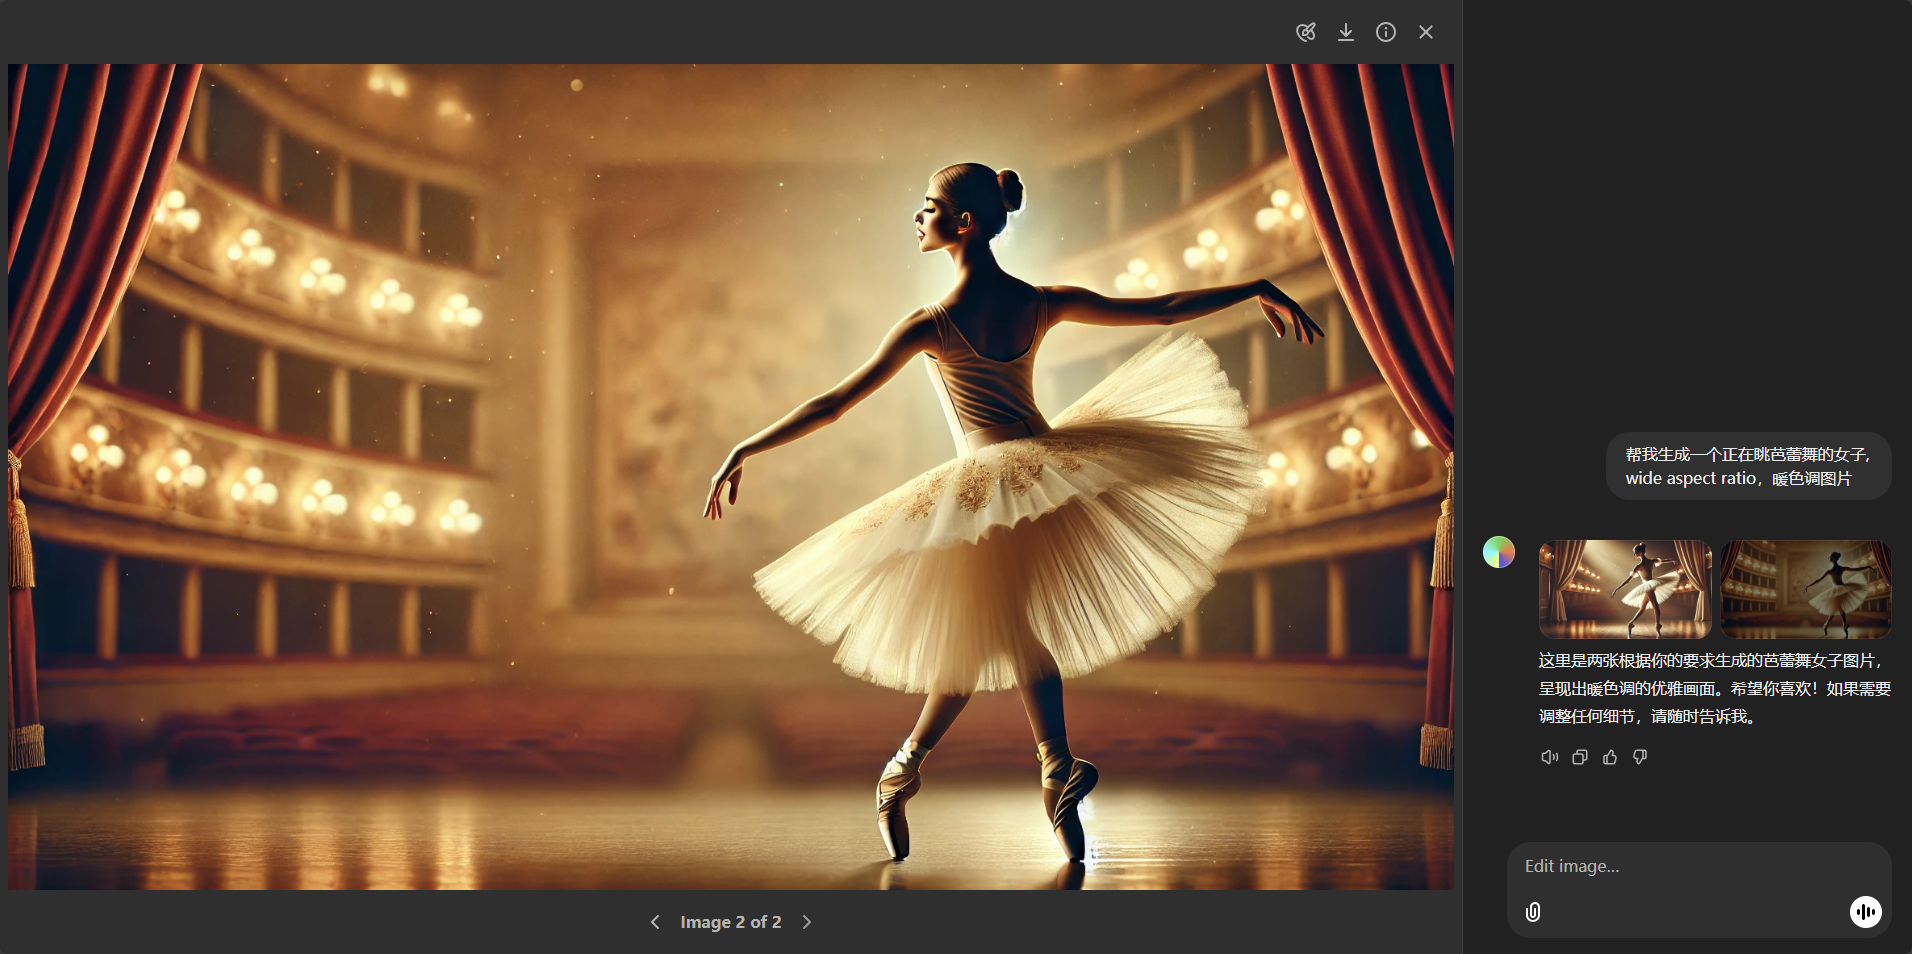
\includegraphics[width=\linewidth]{image/4/DELL图像生成.png}
  \caption{使用人工智能工具生成的正在跳芭蕾舞的女子}
  \label{fig:DELL图像生成}
\end{figure}

此外,人工智能在图像编辑和修复方面也展示了强大的能力。基于深度学习的图像生成模型能够自动修复损坏的照片、调整图像的光影效果,甚至生成高分辨率的图像。这种技术的广泛应用可能会重新定义视觉艺术创作的范畴,减少设计师的工作负担,同时也赋予视觉创作更大的创意空间。

OpenAI与其他机构合作发布的图像生成模型,能够根据复杂的文本提示生成高质量的图像,并支持用户对生成结果进行细致的调整。这些模型的技术原理主要包含编码和生成两个步骤,利用扩散模型的思想,从简单的噪声信号出发,逐步添加细节和模式,最终生成复杂的新数据。这些能力使其成为图像设计和视觉创作中一个强大的工具,能够辅助设计师在创作过程中快速生成概念图、广告素材等,提高创作效率并降低成本。


\paragraph{生成影视}

在影视制作中,生成式人工智能的应用可以改变电影、电视剧的创作和制作方式。人工智能已经能够在多个环节中为导演和制作团队提供创作支持。例如,人工智能可以通过分析已有的剧本、人物对话和情节线索,生成新的剧情和对话,甚至可以根据用户偏好自动推荐可能的剧本发展方向。

生成对抗网络和深度学习模型在影视制作中的应用广泛,尤其是在图像生成和特效制作方面。通过训练人工智能生成器,制作团队可以自动生成特定场景的视觉效果、虚拟人物或逼真的环境。在特效制作中,人工智能可以帮助生成更复杂、更细致的视觉效果,极大地降低制作成本,同时提高制作效率。

生成式人工智能还可以用于电影配乐、音效合成等方面。人工智能通过分析电影的剧情、情感变化和节奏来生成适合的音乐和音效,从而减少人工干预。人工智能甚至可以在虚拟现实\footnote{虚拟现实(Virtual Reality, VR)是一种通过计算机技术创造沉浸式虚拟环境的技术,使用户能够与该环境进行交互。}和增强现实\footnote{增强现实(Augmented Reality, AR)是一种将虚拟信息叠加到现实世界中,以实现交互和信息增强的技术。}场景中自动生成交互式内容,为用户带来更加沉浸式的体验。

特别值得一提的是,OpenAI于2024年2月发布了文生视频大模型,能够仅仅根据提示词生成60秒的连贯视频。该模型将人工智能技术从文本、图像进一步延伸到视频领域。这个模型能够根据用户输入的文本描述自动生成视频内容,这些视频可以包含多个角色、特定类型的运动,以及主题和背景的准确细节。

\begin{figure}[ht]
  \centering
  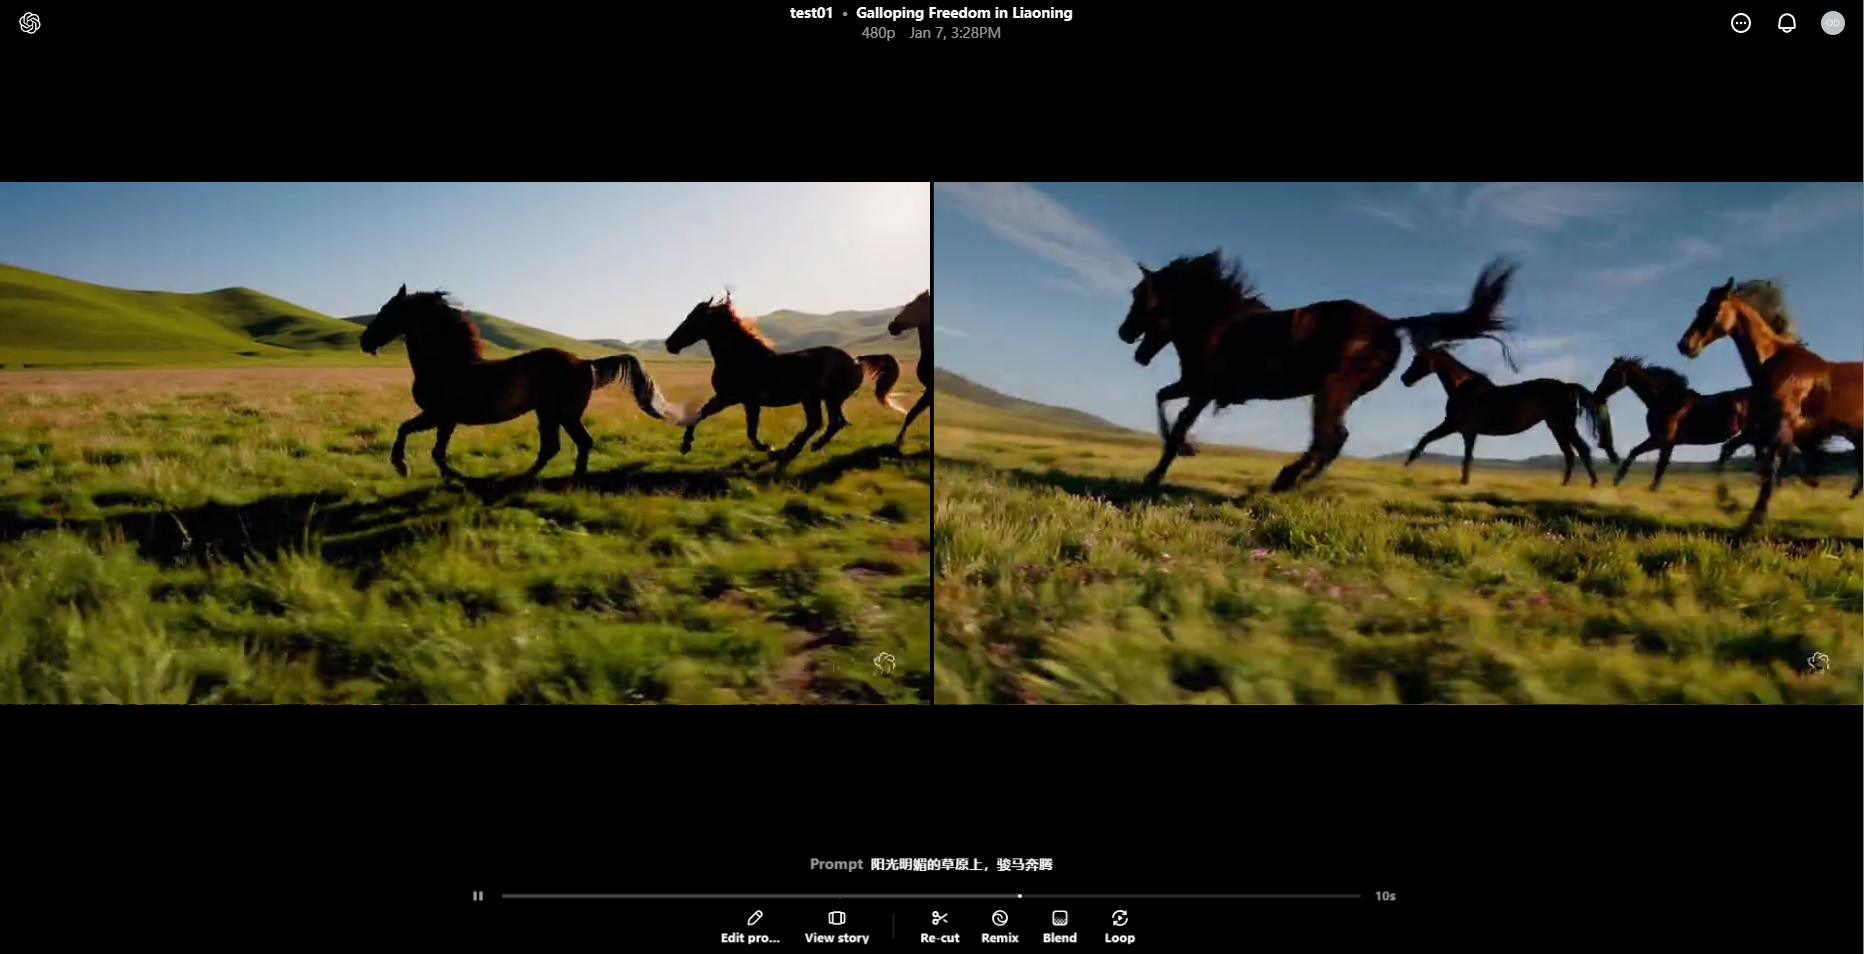
\includegraphics[width=\linewidth]{image/4/sora.png}
  \caption{文生视频}
  \label{fig:sora}
\end{figure}

例如,用户输入一段描述“阳光明媚的草原上,骏马奔腾”的文字,大模型就能生成一个展现该场景的视频。其中的技术原理主要包含编码和生成两个步骤,它利用扩散模型的思想,从简单的噪声信号出发,逐步添加细节和模式,最终生成复杂的新数据。这些能力使其成为影视制作中一个强大的工具,能够辅助导演和制作团队在创作和特效制作等多个环节,提高效率并降低成本。

\paragraph{生成式人工智能对娱乐产业的影响}

% 生成式人工智能的广泛应用正在改变娱乐产业的生产方式。首先,人工智能降低了创作和制作的门槛,使得更多的创作者可以利用人工智能工具进行创作,无论是音乐、影视还是游戏等领域。其次,生成式人工智能极大提高了生产效率,减少了创作所需的时间和成本。例如,人工智能可以自动生成背景音乐、剧本创意、虚拟人物等,大大缩短了创作周期。

% 然而,人工智能创作也带来了一些挑战,尤其是在版权和原创性方面。人工智能生成的内容与传统创作的作品可能存在显著差异,如何界定人工智能创作的版权、以及如何评估其创作的原创性,成为了娱乐产业面临的重要问题。未来,如何合理调整版权法和伦理标准,将是解决这一问题的关键。

生成式人工智能的广泛应用正在改变娱乐产业的生产方式。首先,人工智能降低了创作和制作的门槛,使得更多的创作者可以利用人工智能工具进行创作,无论是音乐、影视还是游戏等领域。其次,生成式人工智能极大提高了生产效率,减少了创作所需的时间和成本。例如,人工智能可以自动生成背景音乐、剧本创意、虚拟人物等,大大缩短了创作周期。

在电影制作领域,生成式人工智能的应用尤为突出。以电影《阿凡达》为例,导演詹姆斯·卡梅隆(James Cameron)使用了先进的动作捕捉和面部捕捉技术,将真人演员的表演转化为虚拟角色的动作和表情。这种技术不仅使角色的动作和表情更加自然和真实,还极大地提高了制作效率。通过头戴式摄像头和改进的软件算法,演员的面部表情被高精度地采集并应用于虚拟角色,从而创造出令人惊叹的外星生物形象。这种技术的应用不仅降低了制作成本,还为电影制作提供了更多的创意空间。
在电影《流浪地球3》中,生成式人工智能在前期阶段被系统性地应用,帮助创作团队快速生成视觉内容和剧本创意,从而加速了项目的开发进程。

其次,在音乐产业中,使用数字人技术\footnote{数字人技术是指利用计算机图形学、人工智能和虚拟现实等技术创建和模拟虚拟人类形象及其行为的领域。}可以打造虚拟偶像,进行音乐创作、表演和互动。腾讯打造的虚拟偶像星瞳,不仅在哔哩哔哩平台进行虚拟直播,还与音乐、体育等领域展开跨界合作,探索数字人的更多可能性。数字人偶像可以24小时不间断地进行表演,不受真人偶像的限制,同时也能与粉丝进行更直接的互动,增强粉丝的参与感和忠诚度。

然而,人工智能创作也带来了一些挑战,尤其是在版权和原创性方面。人工智能生成的内容与传统创作的作品可能存在显著差异,如何界定人工智能创作的版权、以及如何评估其创作的原创性,成为了娱乐产业面临的重要问题。未来,如何合理调整版权法和伦理标准,将是解决这一问题的关键。

\subsubsection{3.小结}

智能娱乐与个性化推荐系统通过分析用户行为和兴趣,为每个用户提供量身定制的娱乐内容推荐。推荐算法(包括协同过滤、内容推荐和混合推荐等)基于用户的历史行为、物品的属性以及其他多维度的数据,为用户提供更精准的推荐。生成式人工智能的应用使得娱乐内容的创作变得更加创新和高效,在音乐、影视等领域带来了前所未有的变革。尽管如此,生成式人工智能在版权和原创性等方面仍面临一些挑战,需要在未来得到合理解决。


\section{智慧驾驶}

在智能驾驶技术的推动下,自动驾驶成为智慧交通的重要组成部分,代表着未来出行方式的革命性转变。随着计算机视觉和深度学习技术的不断发展,自动驾驶系统在环境感知、障碍物识别、决策控制等方面取得了显著进展,能够有效提高驾驶安全性与效率,并逐步推动交通系统的智能化。具体而言,计算机视觉为车辆提供了精准的周边环境理解,而深度学习则赋予系统更强的自主决策能力。自动驾驶技术的持续发展,将促进交通系统向更高效、更安全、更环保的方向迈进,推动智能城市与智慧交通的全面实现。

\subsection{自动驾驶技术}

自动驾驶技术是智慧驾驶领域的核心组成部分,旨在通过先进的传感器、计算机视觉和深度学习技术,实现车辆的自主导航和控制。该技术不仅提高了驾驶的安全性和效率,还为未来的交通系统带来了革命性的变革。以下将详细介绍计算机视觉在自动驾驶中的应用、深度学习在自动驾驶决策系统中的关键作用,并通过实际案例分析自动驾驶技术在日常生活中的应用。

\subsubsection{1.计算机视觉在自动驾驶中的应用}

在自动驾驶系统中计算机视觉技术扮演着至关重要的角色,其主要任务是让车辆能够“看懂”周围环境,识别并理解各种交通元素,从而做出安全的驾驶决策。具体应用包括环境感知、障碍物检测与识别、道路标志识别、行人检测以及路径规划等。

\begin{figure}[ht]
  \centering
  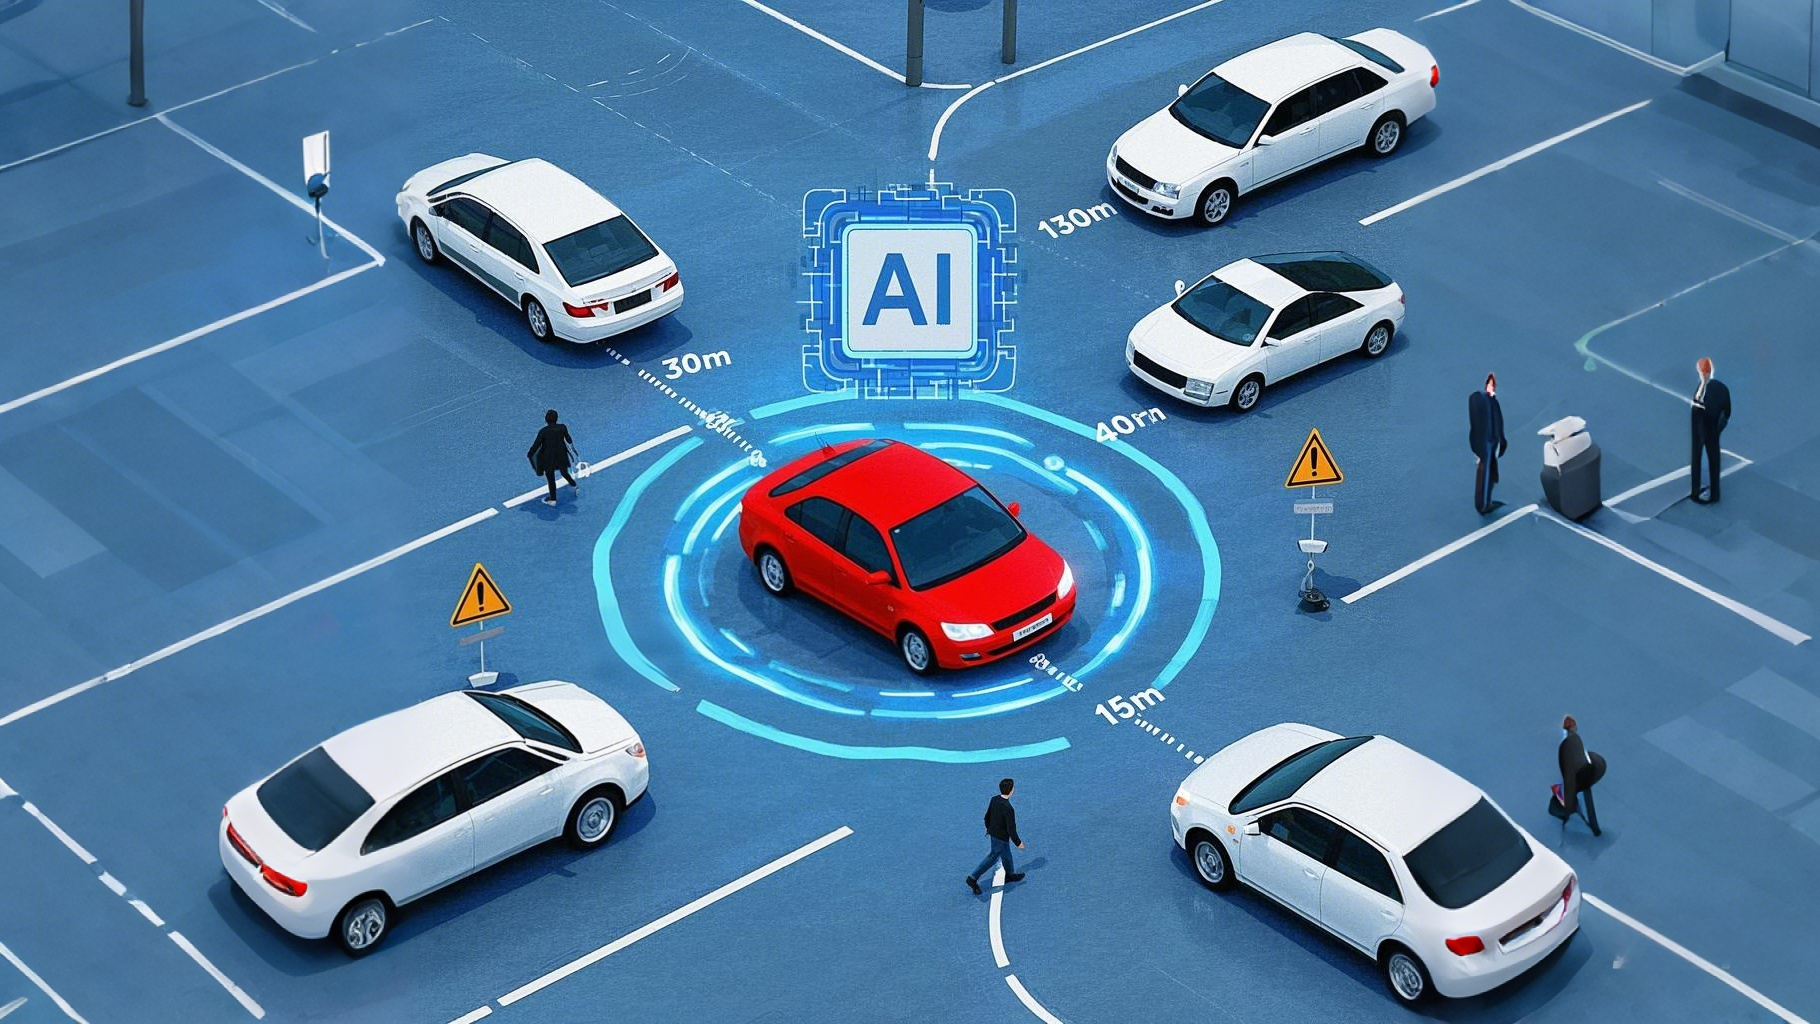
\includegraphics[width=\linewidth]{image/4/新_智能驾驶.png}
  \caption{智能驾驶示意图(图片由AI生成)}
  \label{fig:智能驾驶}
\end{figure}

\textbf{环境感知}是自动驾驶车辆理解其周围环境的基础,依赖于多种传感器(如摄像头、雷达、激光雷达)获取的视觉数据。计算机视觉技术通过处理这些数据,构建车辆周围的三维环境模型。摄像头捕捉到的图像首先进行预处理,包括去噪、色彩校正和图像增强,以提高后续分析的准确性。利用卷积神经网络等深度学习模型,从图像中提取关键特征,如边缘、纹理和形状等。将提取的特征用于构建车辆周围环境的三维模型,识别道路、障碍物、行人和其他车辆的位置和状态。

\textbf{障碍物检测与识别}是确保自动驾驶车辆安全行驶的重要环节。计算机视觉通过深度学习算法,能够准确识别和分类道路上的各种障碍物,包括静止物体(如路障、停放车辆)和动态物体(如行人、自行车、其他机动车辆)。使用深度学习模型在实时视频流中检测和定位障碍物的位置。对检测到的障碍物进行分类,区分行人、车辆、动物等不同类别,以便采取相应的驾驶策略。通过分析动态障碍物的运动轨迹,预测其未来的位置和行为,辅助决策系统制定避让策略。

\textbf{道路标志识别}是自动驾驶车辆遵守交通规则的重要保障。计算机视觉技术能够实时识别并理解各种交通标志,如限速标志、停车标志、禁行标志等。首先,利用深度学习模型在图像中检测交通标志的位置。其次,对检测到的标志进行分类,识别其具体含义和指示内容。最后,将识别到的交通标志信息与车辆的导航系统相结合,调整驾驶行为以符合交通规则。

\textbf{行人检测}是确保自动驾驶车辆行驶安全的关键技术之一。计算机视觉通过深度学习模型,能够准确检测和跟踪行人位置,预防潜在的碰撞风险。使用深度学习算法在实时视频中检测行人的存在。通过多目标跟踪算法,持续跟踪行人的位置和运动轨迹。分析行人的行为模式,预测其可能的移动路径,辅助车辆做出及时的避让决策。

\textbf{路径规划}是自动驾驶系统中决定车辆行驶路线的重要环节。计算机视觉提供的环境感知数据与深度学习算法相结合,能够生成安全、高效的行驶路径。基于环境感知数据,利用深度学习模型生成候选行驶路径。通过强化学习等算法,对候选路径进行评估和优化,选择最优行驶路线。根据动态环境变化,实时调整路径规划,确保车辆始终处于最佳行驶状态。

无人驾驶技术已经广泛应用到人们的日常生活中,比如,由某公司推出的一款自动驾驶汽车服务,展示了计算机视觉和深度学习技术在自动驾驶领域的实际应用。项目中采用了多种传感器融合技术,包括高清摄像头、激光雷达和毫米波雷达,以实现高精度的环境感知。通过先进的深度学习算法,能够实时检测和识别道路标志、行人及其他车辆,确保行驶的安全性。

此外,该项目还引入了强化学习算法,用于优化车辆的决策和控制系统,使其能够在复杂的城市交通环境中自主导航和避让障碍物。该项目不仅展示了计算机视觉在自动驾驶中的关键作用,也突显了深度学习在决策系统中的重要性,为未来自动驾驶技术的发展提供了宝贵的实践经验。

特斯拉的自动驾驶技术(Autopilot)是业界领先的自动驾驶解决方案之一,广泛应用于其电动汽车系列中。Autopilot系统依赖于一系列高分辨率摄像头、超声波传感器和雷达,结合强大的计算能力和深度学习算法,实现车辆的自主驾驶功能。
特斯拉Autopilot的核心技术包括视觉感知、路径规划与控制、自动变道与导航和自适应巡航控制\footnote{自适应巡航控制(Adaptive Cruise Control, ACC)是一种自动驾驶辅助系统,能够根据前方车辆的速度自动调整自身车速,以保持安全的跟车距离。}等。

特斯拉不断通过OTA(Over-The-Air)\footnote{OTA(Over-The-Air)指的是一种通过无线网络远程更新软件或固件的技术。OTA更新使得Autopilot系统能够不断优化和提升其性能,而无需车主手动进行更新。这种方式依赖于大规模的数据收集和深度学习,确保系统在各种驾驶场景中具备更好的适应性和可靠性。}更新优化Autopilot系统,提升其环境感知和决策能力。通过大规模的数据收集和深度学习模型的持续训练,Autopilot系统在不同驾驶场景下展现出卓越的适应性和可靠性,推动了自动驾驶技术的普及与发展。

\subsubsection{2.自动驾驶决策系统}

% 在自动驾驶决策系统中深度学习发挥着核心作用,通过处理大量的传感器数据,帮助车辆做出智能化的驾驶决策。深度学习技术不仅提升了车辆对复杂环境的理解能力,还增强了其自主决策和适应能力。

% 自动驾驶决策系统的基础是深度神经网络,通过多层次的网络结构,深度神经网络能够处理和分析来自不同传感器的数据,实现复杂的决策任务。主要应用包括车辆控制、导航与路径规划以及行为预测。具体来说,利用深度神经网络模型,根据环境感知数据,实时调整车辆的加速、制动和转向,实现平稳、安全的驾驶。基于深度学习算法,自动驾驶系统能够生成和优化行驶路径,避开障碍物,选择最优路线。通过分析其他道路使用者的行为模式,预测其未来的行动,确保行驶安全。

% 强化学习是深度学习在自动驾驶决策中的一种重要应用,通过试错学习,强化学习算法能够优化驾驶策略,提高自动驾驶系统的适应性和安全性。具体应用包括策略优化、自适应控制和应急响应。强化学习算法通过与环境的交互,不断优化驾驶策略,学习如何在不同的交通场景中做出最佳决策。在复杂多变的交通环境中,强化学习算法能够根据实时反馈,动态调整车辆的控制策略,适应不同的行驶条件。在突发情况下,强化学习算法能够迅速做出反应,采取有效的应急措施,避免潜在的交通事故。

% 在自动驾驶决策系统中,通过多传感器数据融合技术,提升了车辆对环境的感知和理解能力。通过整合来自摄像头、雷达、激光雷达等多种传感器的数据,深度学习模型能够生成更加准确和全面的环境认知,支持更复杂的决策任务。具体来说,利用深度学习算法,将不同传感器的数据进行融合,消除数据间的冗余和噪声,提升感知精度。通过统一的深度学习模型,处理多模态数据,实现对环境的全面理解,包括物体检测、分类和跟踪。深度学习模型具备高效的数据处理能力,能够实时分析和处理多传感器数据,支持即时决策和控制。

% 深度学习模型在自动驾驶决策系统中的优化和训练,是提升系统性能和可靠性的关键。通过大规模的数据训练和模型优化,深度学习算法能够不断提升决策系统的智能化水平。首先,利用海量的驾驶数据,对深度学习模型进行训练,涵盖各种驾驶场景和环境条件,增强模型的泛化能力。

% 然后,通过模型剪枝、量化和并行计算等技术\footnote{模型剪枝是指通过去除神经网络中不重要的权重或节点来减少模型的大小和计算复杂度,量化是将模型中的浮点数参数转换为低精度表示以降低存储和计算需求,而并行计算是同时利用多个计算单元加速模型的训练和推理过程。},优化深度学习模型的结构和性能,提高决策系统的响应速度和准确性。最后,深度学习模型能够通过持续学习和在线更新,不断适应新的驾驶环境和用户需求,提升自动驾驶系统的智能化和适应性。

自动驾驶决策系统的核心在于如何让车辆在复杂的交通环境中做出智能化的驾驶决策。其实现主要依赖于深度学习,通过对大量传感器数据的分析,帮助车辆理解周围环境并做出相应的反应。深度学习不仅提升了车辆对复杂场景的识别能力,还增强了其自主决策和适应不同驾驶条件的能力。

自动驾驶决策系统的基础是深度神经网络,这种网络结构能够综合来自多种传感器的信息,进行全面的环境感知和分析。通过深度神经网络,车辆可以实时调整加速、制动和转向,实现平稳且安全的驾驶。此外,系统还能够规划最佳行驶路径,避开障碍物,并预测其他道路使用者的行为,确保行车安全。

在决策过程中,强化学习发挥了重要作用。通过不断与环境互动,强化学习算法能够优化驾驶策略,使车辆在各种交通场景中做出最优决策。无论是在繁忙的市区还是高速公路,系统都能根据实时反馈动态调整控制策略,适应不同的行驶条件。在突发情况下,强化学习算法还能迅速做出反应,采取有效的应急措施,避免潜在的交通事故。

多传感器数据融合技术是提升自动驾驶决策系统感知能力的关键。通过整合来自摄像头、雷达和激光雷达等多种传感器的信息,系统能够形成对环境的全面理解。这种数据融合不仅提高了感知的准确性,还支持更复杂的决策任务,使车辆能够在多变的道路环境中保持高效和安全的运行。

为了确保决策系统的高效性和可靠性,深度学习模型需要经过大量的数据训练和优化。通过不断的学习和调整,系统能够适应新的驾驶环境和用户需求,提升整体智能化水平。持续的模型优化和更新,使得自动驾驶决策系统在面对不同的驾驶挑战时,能够表现出更高的适应性和安全性。

总之,自动驾驶决策系统通过深度学习和强化学习等先进技术,实现了对复杂交通环境的精准感知和智能决策,为未来的智能交通提供了坚实的技术支持。

\subsubsection{3.SAE 分级标准}
SAE分级是由美国汽车工程师协会(Society of Automotive Engineers,SAE)制定的自动驾驶技术等级标准,用于划分自动驾驶系统的不同发展阶段。该分级标准从0到5,共分为六个等级,主要依据自动驾驶系统中人类驾驶员介入的程度来区分。了解SAE分级有助于评估自动驾驶技术的发展水平和实际应用能力。

0级(无自动化)是指完全由人类驾驶员控制,没有任何自动化。在这一等级下,驾驶员需要全程控制车辆。

1级(驾驶辅助)则是车辆提供某些辅助功能,通常是单一功能(如自适应巡航控制或车道保持),但驾驶员仍需控制大部分驾驶任务,只是可以使用辅助功能来减轻负担。

2级(部分自动化)意味着车辆可以同时执行多个任务,如自适应巡航控制和车道保持控制,但驾驶员仍然需要保持注意力,并随时准备接管控制。

3级(有条件自动化)是在某些条件下,车辆可以完全控制所有驾驶任务,驾驶员可以将注意力转移到其他活动上,但在系统请求时需要及时介入。此时,在特定环境(如高速公路)下,自动驾驶系统可以执行所有任务,但驾驶员必须迅速响应接管请求。

4级(高度自动化)表示车辆可以在特定的环境或情况下完成所有驾驶任务,驾驶员不再需要参与控制。在此级别下,自动驾驶系统能够在如城市道路或特定地理区域内全权负责驾驶,即使驾驶员没有准备好介入。

5级(完全自动化)则是车辆能够在所有环境和情况下完成所有驾驶任务,无需驾驶员介入,车辆可以在任何环境下自我驾驶,完全实现无人驾驶。

\begin{figure}[ht]
  \centering
  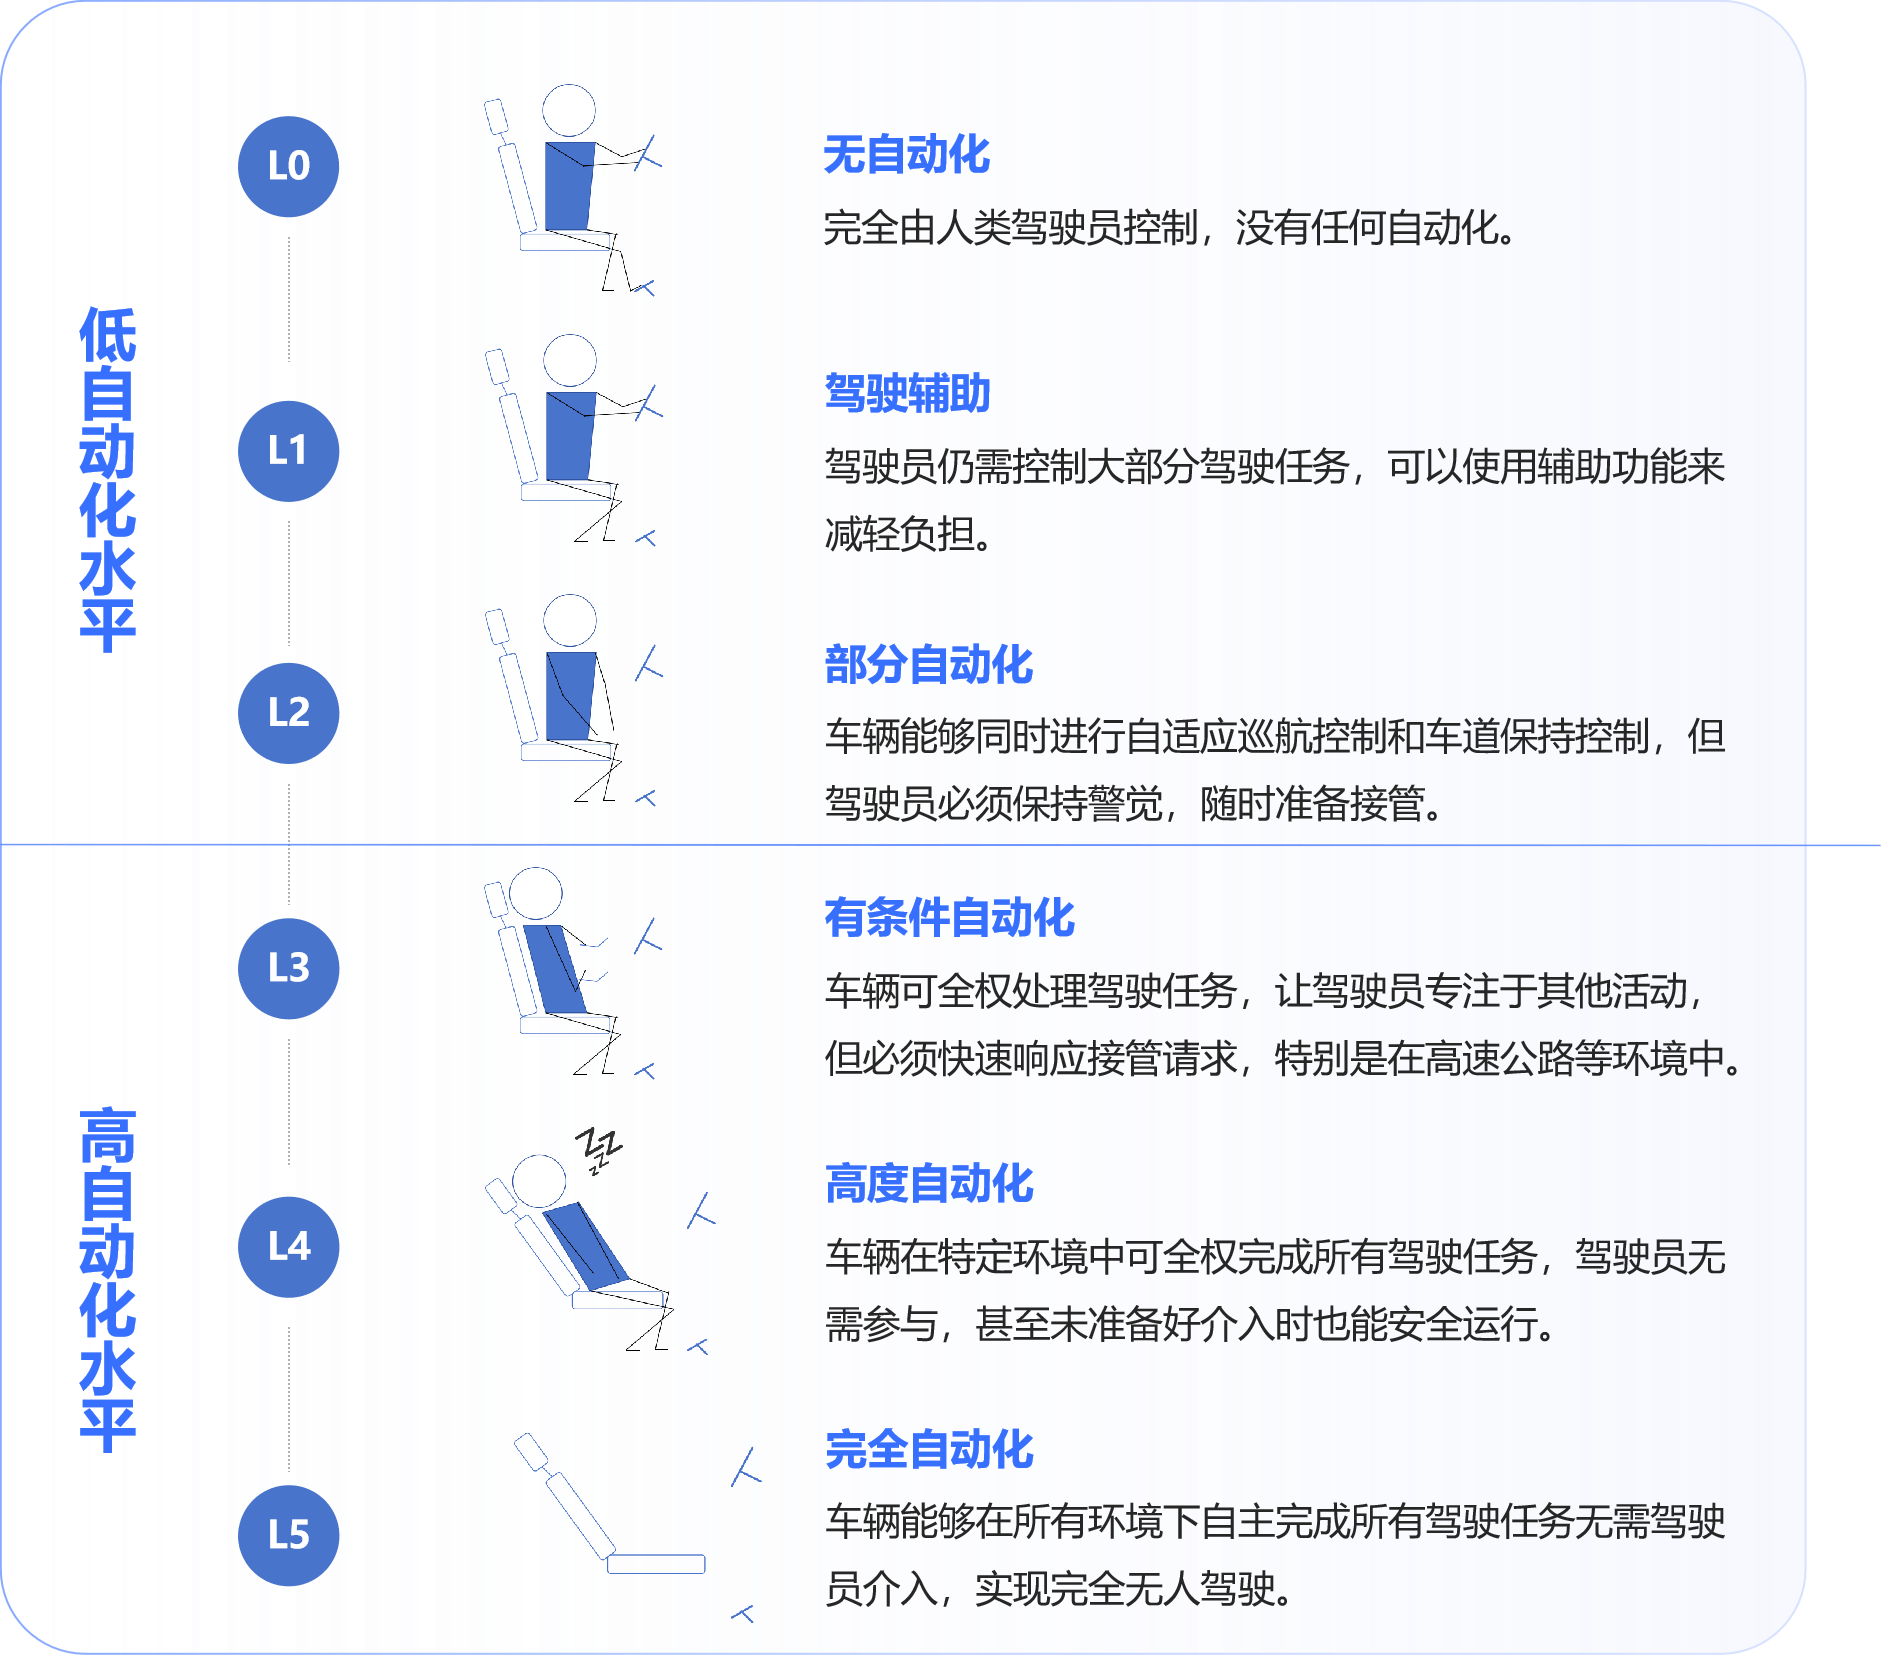
\includegraphics[width=0.95\linewidth]{image/4/自动驾驶等级.png}
  \caption{SAE分级示意图}
  \label{fig:SAE分级}
\end{figure}

SAE的分级帮助行业、法规制定者和消费者更好地理解自动驾驶技术的进展和不同系统的能力,确保安全和逐步实施自动驾驶技术。理解SAE分级标准有助于评估不同自动驾驶系统的功能和限制,指导技术研发和市场推广。

\subsubsection{4.未来发展趋势}
未来,自动驾驶技术将继续朝着更高的智能化和自主化方向发展,具体体现在更高精度的环境感知、更加智能的决策系统、多模态数据融合以及车联网与协同驾驶等方面。

随着传感器技术和计算机视觉算法的不断进步,自动驾驶车辆将具备更高精度的环境感知能力,能够在更加复杂和动态的交通环境中安全行驶。同时,深度学习和强化学习算法的持续优化将使自动驾驶决策系统更加智能,能够应对更多样化和突发性的交通状况。

\subsubsection{5.小结}

自动驾驶技术通过计算机视觉和深度学习的深度结合,实现了车辆的自主导航和控制。计算机视觉技术负责环境感知和障碍物检测,为深度学习决策系统提供了精准的数据支持;而深度学习技术则通过分析和处理这些数据,做出智能化的驾驶决策,确保行驶的安全性和效率。SAE分级标准进一步明确了自动驾驶技术的发展阶段和能力范围。随着技术的不断进步,自动驾驶系统将变得更加智能和可靠,推动未来交通系统向更加安全、高效和环保的方向发展。

\subsection{车联网与智能交通管理}

车联网(Vehicle-to-Everything,V2X)技术和智能交通管理系统(Intelligent Transportation Systems,ITS)是智慧驾驶领域的重要组成部分,旨在通过先进的通信技术和人工智能算法,实现车辆与车辆、车辆与基础设施之间的高效协作与信息共享,从而优化交通流量、提升交通安全性并提高应急响应效率。以下将详细介绍车联网技术的工作原理及其在交通管理中的应用,以及智能交通系统中人工智能技术在交通流量优化、事故预防与应急响应中的具体应用。

\begin{figure}[ht]
  \centering
  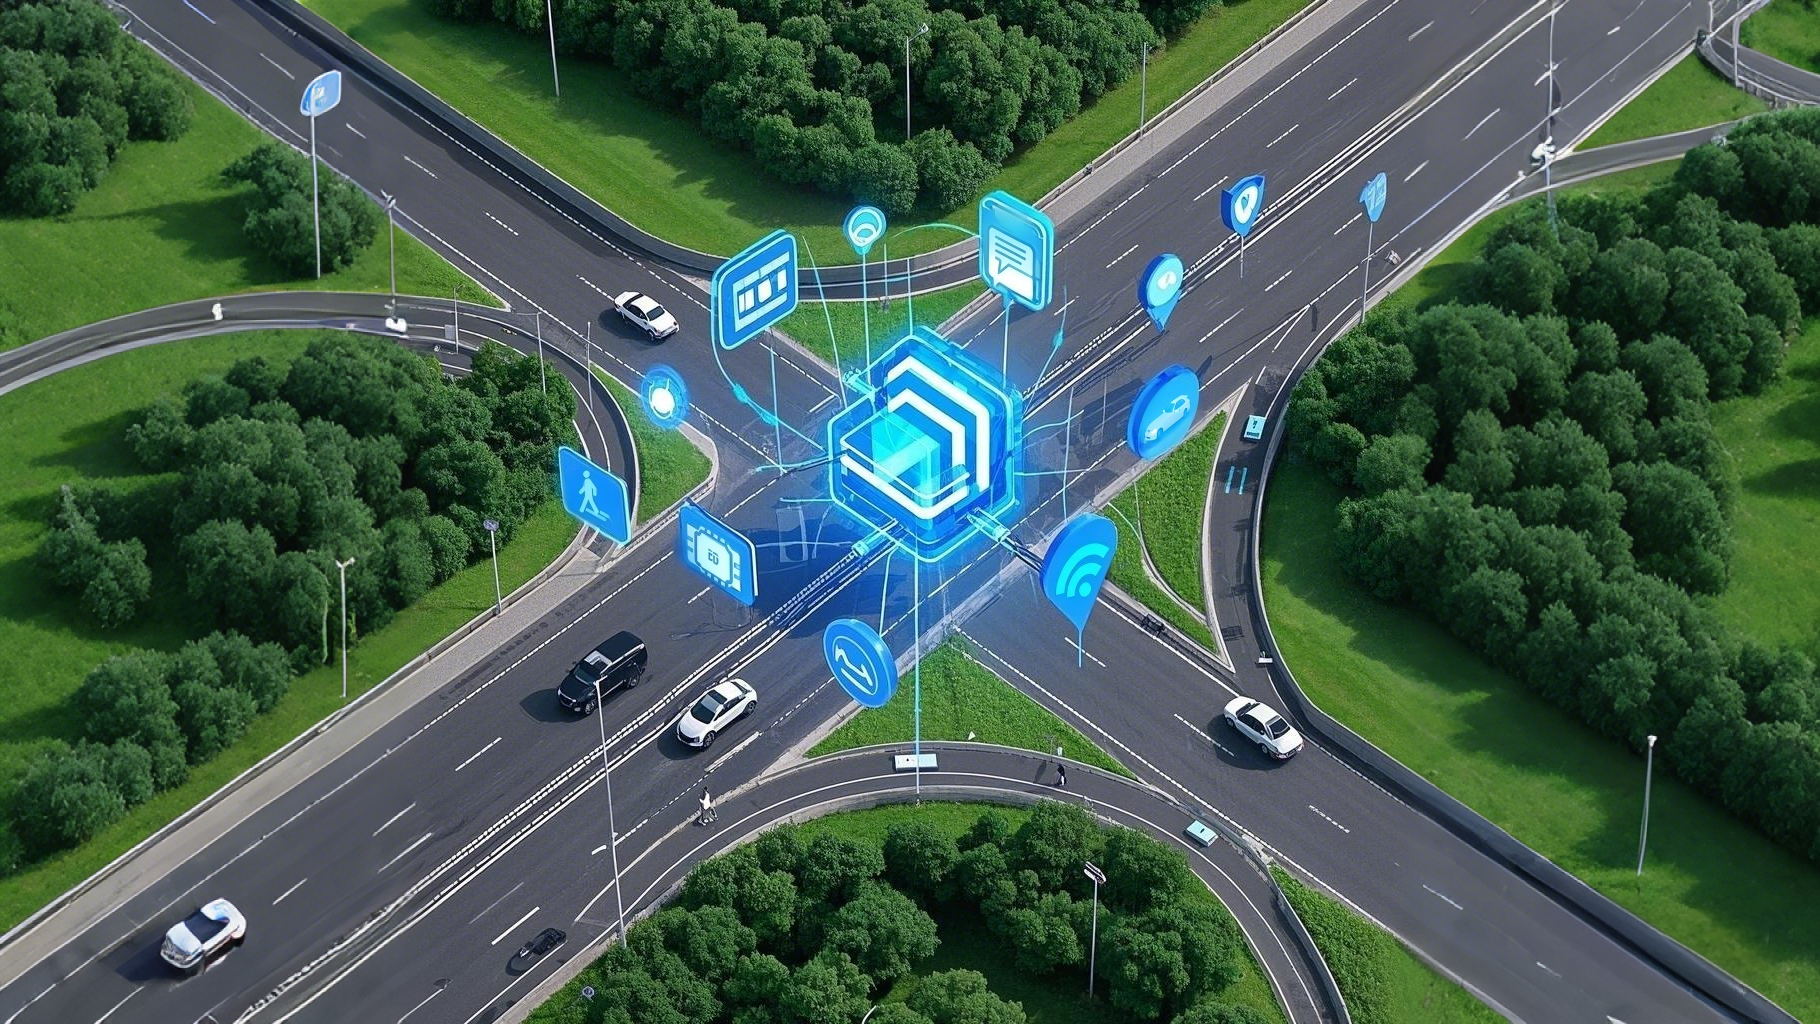
\includegraphics[width=\linewidth]{image/4/新_智能交通.png}
  \caption{车联网与智能交通管理(图片由AI生成)}
  \label{fig:智能交通}
\end{figure}

\subsubsection{1.车联网(V2X)技术}

车联网技术通过实现车辆与外部环境的实时通信,显著增强了车辆的感知能力和决策能力,从而提高了整个交通系统的效率和安全性。在车联网技术中,车辆之间以及车辆与基础设施、行人之间的多种通信模式发挥着关键作用。

首先,车辆之间的直接信息交换,即V2V(Vehicle-to-Vehicle)通信,是车联网的核心组成部分。通过V2V通信,车辆可以共享诸如速度、位置、加速度和转向角度等动态信息。这种实时的信息共享使得车辆能够提前感知周围环境中的潜在危险,例如前方车辆突然制动或并线的情况,从而实现协同驾驶和有效的碰撞预防,显著提升行车安全性。

其次,车辆与道路基础设施之间的通信,即V2I(Vehicle-to-Infrastructure)通信,同样至关重要。通过V2I通信,车辆能够接收到来自交通信号灯、道路传感器、收费站等基础设施的实时信息。这些信息包括交通信号的当前状态、道路施工情况以及交通拥堵状况等。基于这些数据,车辆可以优化行驶路线和速度,减少交通拥堵,提高行车效率,进而提升整体交通系统的运行效率。

此外,车辆与行人之间的通信,即V2P(Vehicle-to-Pedestrian)通信,也在车联网中占据重要地位。通过智能手机或可穿戴设备,行人的位置信息和运动状态可以实时传输给周围的车辆。车辆根据这些信息调整行驶行为,如减速或停车,以避免与行人发生事故,从而大幅提高行人安全性。

综上所述,车联网技术通过多种通信模式的协同作用,不仅提升了车辆的感知和决策能力,还优化了交通流量和行车安全。随着技术的不断进步,车联网将在智慧交通和智能城市的发展中发挥越来越重要的作用,为人们提供更加高效、安全和便捷的出行体验。

\subsubsection{2.智能交通系统}

智能交通系统通过整合车联网技术和人工智能算法,实现了交通管理的智能化和自动化。智能交通系统的主要目标包括优化交通流量、提升交通安全性、减少交通拥堵以及提高应急响应效率。人工智能在智能交通系统中的具体应用十分广泛。

\textbf{在交通流量优化方面},人工智能技术通过实时分析交通数据,优化交通信号灯的控制和交通流量管理,从而提高道路使用效率,减少车辆等待时间和燃油消耗。例如,智能交通信号控制利用机器学习算法分析交通流量数据,动态调整交通信号灯的时长和配时策略,以适应不同时间段和交通状况。

人工智能驱动的交通信号控制系统根据实时交通流量自动优化信号配时,有效缓解了高峰时段的交通拥堵。此外,人工智能算法结合实时交通信息,为驾驶员提供最优行驶路线建议,避免拥堵区域,缩短行驶时间。像Google Maps和高德地图这样的导航应用利用人工智能技术,根据实时交通数据动态调整路线,显著提升了用户的出行体验。

\textbf{在事故预防方面},人工智能技术通过分析历史交通事故数据和实时交通信息,能够预测潜在的事故风险并采取预防措施,从而显著提升交通安全性。危险区域识别与警示功能利用深度学习算法分析交通监控视频,识别事故高发区域,并实时发布警示信息给驾驶员和交通管理部门。

例如,一些智能交通系统通过人工智能分析监控视频,自动识别视线不良或交通复杂的路段,提前发布警告,减少事故发生率。同时,人工智能系统还可以监测驾驶员的驾驶行为,如疲劳驾驶和酒驾,通过实时分析提供警示和干预措施,防止因驾驶员行为不当导致的事故。例如,自动驾驶系统通过人工智能技术监测驾驶员的注意力状态,必要时发出警告,提示驾驶员集中注意力。

\textbf{在应急响应方面},人工智能技术发挥着关键作用,通过快速分析和处理交通事故或灾害现场的数据,优化应急资源的调度和部署,提高应急响应的效率和效果。智能应急调度系统利用人工智能算法分析事故现场的实时数据,自动规划救援路线,调度最合适的救援车辆和人员,确保迅速到达事故现场。

例如,一些城市的智能应急调度系统通过人工智能分析事故报告和交通状况,自动分配救援资源,提高救援效率。此外,灾害预测与预警功能通过大数据分析和机器学习模型,预测交通灾害的发生概率,并提前发布预警信息,采取预防措施,减少灾害带来的损失。如,人工智能系统可以根据天气数据和交通流量预测恶劣天气下的交通风险,提前发布警报,提醒驾驶员采取相应措施。

北京市中关村核心区域的智能信号灯控制系统就是一个典型的应用实例。该系统通过高清摄像头、地磁传感器等设备实时捕捉车辆通行数据,包括车流量、车速、车辆类型等信息。人工智能算法对这些数据进行实时处理,构建起路口交通流量的动态模型,动态调整绿灯时长,减少车辆等待时间,提升通行能力。同时,C-V2X车联网技术\footnote{C-V2X (Cellular Vehicle-to-Everything)车联网技术是一种基于蜂窝网络的车用无线通信技术,可实现车辆与周围环境,包括其他车辆、基础设施、行人以及网络之间的全方位通信。}提供了跨车辆、跨路侧设施、跨云端的协同网络,有效解决了“鬼探头”和十字路口盲区碰撞预警等问题,避免了交通事故。在交通效率方面,车联网技术通过智能化的交通管理和资源分配,显著提升了道路的使用效率。

\subsubsection{小结}

车联网技术和智能交通管理系统通过先进的通信技术和人工智能算法,实现了车辆与车辆、车辆与基础设施之间的高效信息共享与协作,显著优化了交通流量、提升了交通安全性并提高了应急响应效率。

车联网技术通过V2V、V2I和V2P通信模式,增强了车辆的感知能力和决策能力,支持智能交通系统在交通流量优化、事故预防与应急响应等方面的应用。智能交通系统利用人工智能技术分析和处理大量交通数据,实现智能化的交通管理与控制,提升了交通系统的整体效率和安全性。

随着通信技术和人工智能算法的不断发展,车联网与智能交通管理系统将在未来智慧城市建设中发挥更加重要的作用,推动交通系统向更加智能、高效和安全的方向发展。


\section{智慧医疗}

智慧医疗代表了医疗行业与人工智能技术深度融合的未来图景,通过计算机视觉、深度学习、自然语言处理等核心技术,为医疗影像分析与诊断支持、个性化医疗与基因分析以及远程医疗与虚拟健康助手等领域带来革新性进展。通过精确的病灶检测、自动化报告生成、个性化治疗方案推荐以及远程诊断和智能健康管理,智慧医疗极大地提升了医疗服务的效率与质量,为患者提供更加精准、高效和个性化的诊疗与健康管理体验。以下内容将深入探讨智慧医疗在影像分析、基因分析和远程医疗等方面的具体应用及其技术实现。

\subsection{医疗影像分析与诊断支持}

随着人工智能技术的飞速发展,医疗领域,特别是医疗影像分析和诊断支持系统,正在经历一场深刻的变革。计算机视觉和深度学习等核心技术在医疗影像中的应用,正逐渐提高疾病早期发现的准确性和效率,同时为医生提供了强有力的辅助支持,改善了患者的诊疗体验。以下将详细探讨计算机视觉在医疗影像分析中的应用,以及人工智能在疾病诊断和治疗决策支持中的作用。

\subsubsection{1.计算机视觉在医疗中的应用}

计算机视觉技术通过模拟和理解人类视觉系统的处理方式,能够自动化地分析和解读医疗影像数据。医疗影像,如X光、磁共振成像(MRI)、计算机断层扫描(CT)等,是诊断疾病、评估治疗效果和进行手术规划的关键工具。人工智能技术,尤其是深度学习和卷积神经网络,已被广泛应用于这些影像的自动分析中,极大地提高了诊断的效率和准确性。

\paragraph{肿瘤检测与病灶识别}

人工智能在肿瘤检测和病灶识别中的应用尤为重要,特别是在早期癌症的诊断中。通过训练深度学习模型,计算机视觉技术可以自动识别影像中的肿瘤或病变区域,帮助医生尽早发现异常并进行进一步分析。例如,计算机视觉技术可用于分析胸部X光片,自动识别肺部结节、肺炎或肺癌等病变。通过与大量标注数据的学习,人工智能能够准确地检测到微小的病变,并与医生的诊断结果进行对比,提高早期肺癌的检测率。在CT或MRI图像中,人工智能模型可以自动分割出脑肿瘤、乳腺癌或其他病变区域,并标注其大小、形状和位置。例如,使用卷积神经网络可以准确识别乳腺影像中的肿块,帮助医生在初期阶段就发现癌症并进行有效干预。

\begin{figure}[ht]
  \centering
  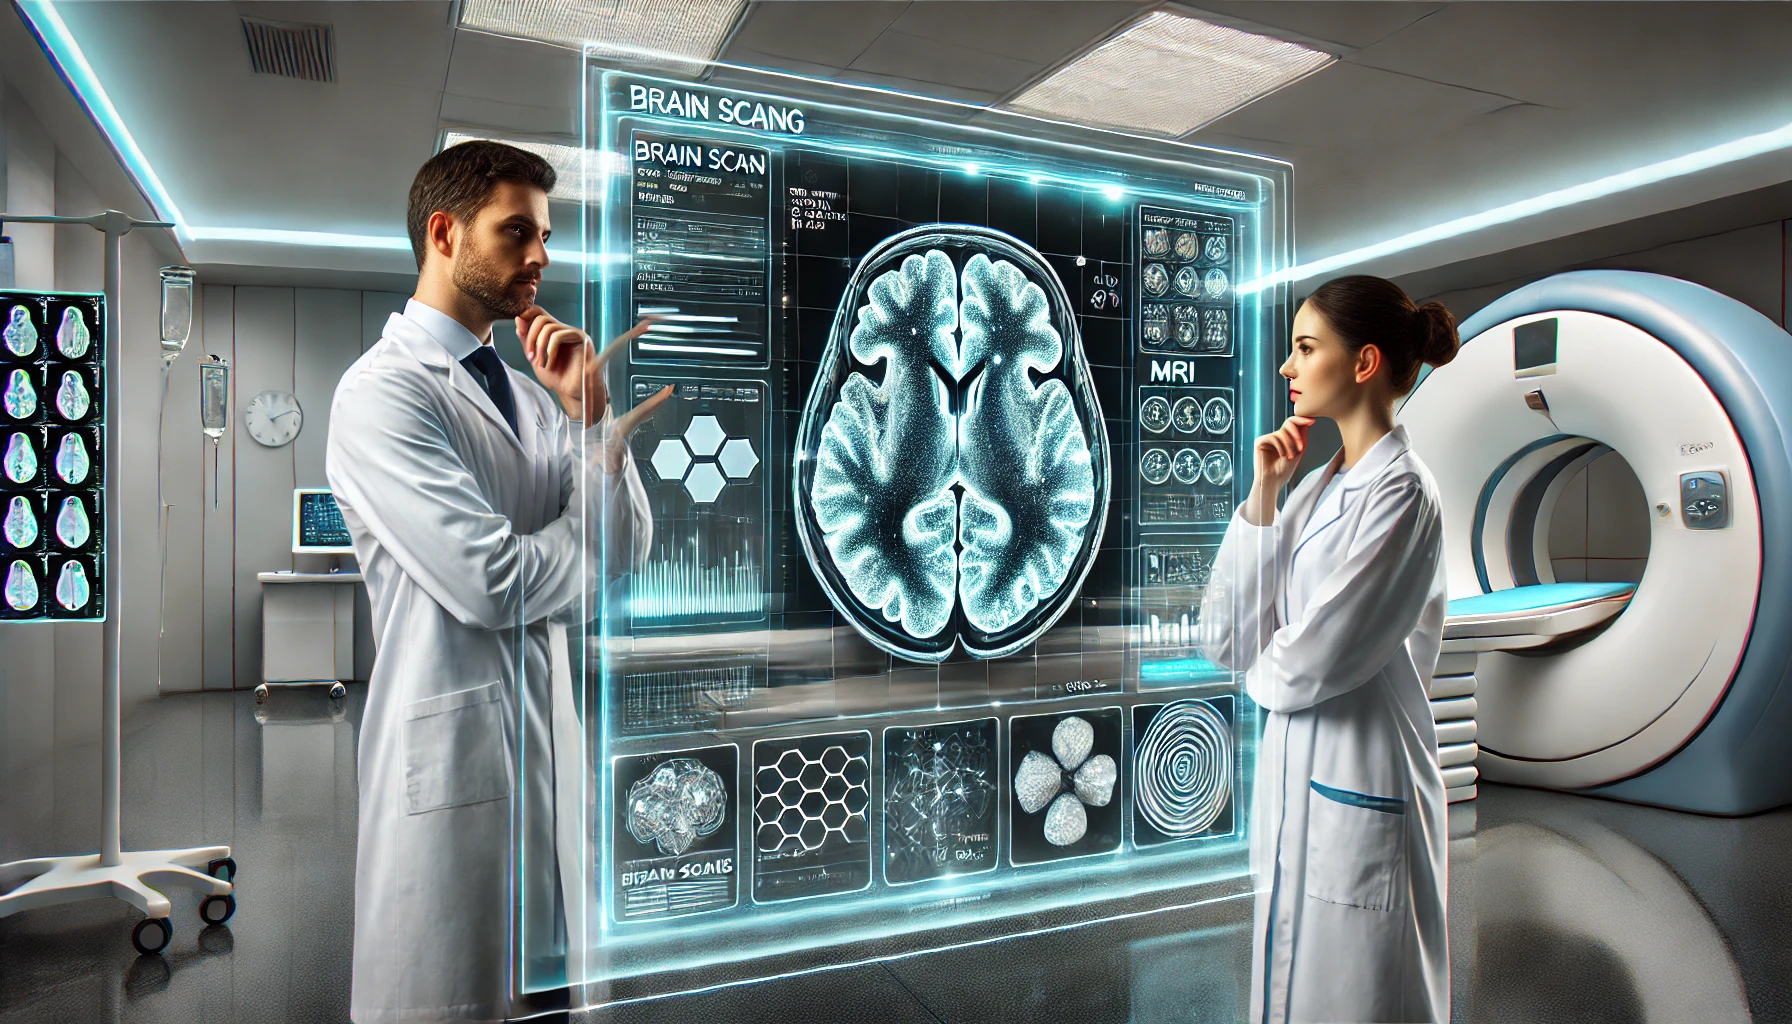
\includegraphics[width=\linewidth]{image/4/医疗影像处理.png}
  \caption{肿瘤病灶影像分析与诊断(图片由AI生成)}
  \label{fig:医疗影像处理}
\end{figure}

这些人工智能技术可以减少人为误差,提升影像分析的精确度,特别是在医生面临大量影像数据时,计算机视觉能够快速筛选出需要关注的区域,大大提高工作效率。

\paragraph{自动化标注与报告生成}

人工智能技术还能够实现影像的自动标注与报告生成,辅助医生生成影像分析报告。例如,在CT扫描中,人工智能可以自动标注出病变区域、计算肿瘤的体积,并生成详细的检测报告。医生可以根据这些自动生成的报告更快地做出诊断决策,从而节省时间并提高诊断质量。

\subsubsection{2.诊断决策支持系统}

人工智能在医学中的另一个重要应用是诊断决策支持系统(Clinical Decision Support System,CDSS)。这类系统通过分析病人的临床数据和影像资料,辅助医生做出更加精准的诊断决策,并根据患者的个体情况提供个性化的治疗方案。

人工智能决策支持系统通常结合患者的病历信息、实验室检查数据和影像数据进行多维度分析。通过深度学习和自然语言处理技术,人工智能能够从患者的电子病历中提取出有价值的信息,并与影像分析结果相结合,为医生提供更加全面和个性化的诊断建议。例如,系统可以分析一名乳腺癌患者的历史病历、家族病史、年龄等因素,并将其与乳腺X光影像进行对比,判断该患者是否有乳腺癌的风险,以及是否需要进一步的检查或治疗。

人工智能还能够根据患者的健康数据预测疾病风险,辅助医生制定个性化的治疗方案。例如,在糖尿病的管理中,人工智能系统通过分析患者的历史就诊数据、生活习惯、饮食偏好等,预测其未来患病的风险,并基于个体化的情况制定饮食、药物和运动等个性化方案。

此外,人工智能可以通过分析大量医学文献、临床试验数据以及患者的治疗历史,推荐最合适的治疗方案或药物。例如,针对癌症患者,人工智能系统能够结合患者的影像数据、基因数据及已有的临床试验成果,提出最适合该患者的治疗方法,从而提升治疗效果。

人工智能决策支持系统能够通过实时提供诊断建议和治疗方案,帮助医生在繁忙的工作中减少遗漏,尤其是在复杂的病例中。当面临多种可能的诊断时,人工智能系统可以分析各种可能性并提供相应的推荐,从而降低误诊率并提高治疗成功率。例如,在急性心肌梗死的诊断中,人工智能通过结合患者的心电图数据、血液检测数据以及影像学资料,帮助医生更精确地判断心脏病发作的类型和程度,进而提出最合适的治疗方案。

\subsubsection{3.小结}

医疗影像分析与诊断支持系统在提升医疗服务质量和效率方面具有重要作用。计算机视觉技术,特别是深度学习与卷积神经网络,在自动化病灶识别、肿瘤检测和影像分析中的应用,为医生提供了强大的辅助支持,能够显著提高诊断准确性和效率。而人工智能驱动的决策支持系统则通过整合患者的多维数据,提供个性化的诊断和治疗建议,进一步提升医疗质量并优化临床决策过程。随着人工智能技术的不断发展,医疗影像分析和诊断支持将成为未来医学实践中不可或缺的一部分,推动医疗领域的智能化、精准化发展。

\subsection{个性化医疗与基因分析}

个性化医疗与基因分析代表了现代医疗发展的前沿,通过对个体基因信息和健康数据的深度解析,实现量身定制的医疗方案。人工智能技术,特别是深度学习、机器学习和自然语言处理,在基因测序、基因数据分析以及疾病风险预测中发挥了关键作用,大幅提升了医疗服务的精准性和效率。以下将详细探讨人工智能在基因数据分析中的应用及其在预测性医疗中的具体应用。

\subsubsection{1.基因数据分析}

基因数据分析利用人工智能技术对大量基因测序数据进行处理和解读,旨在揭示个体基因组的深层信息,从而为个性化医疗提供科学依据。人工智能在基因数据分析中的主要应用包括基因测序自动化、基因变异检测与注释、基因表达分析、多组学数据整合以及个性化治疗方案推荐。

\begin{figure}[ht]
  \centering
  
\includegraphics[width=\linewidth]{image/4/基因测序.png}
  \caption{基因示意图(图片由AI生成)}
  \label{fig:gene}
\end{figure}
\paragraph{基因测序自动化}

% 基因测序是个性化医疗的基础,通过测定个体的DNA序列,了解其基因组信息。传统的基因测序过程复杂且耗时,而人工智能技术的引入显著提高了基因测序的效率和准确性。深度学习算法能够自动化地处理和分析测序数据,减少人为干预,提高测序的通量和质量。

% 例如,人工智能驱动的基因测序平台能够快速识别和校正测序过程中产生的错误,提高测序结果的可靠性。Illumina公司的人工智能算法可以在基因测序过程中实时监控数据质量,自动纠正测序错误,确保高精度的基因组数据输出。此外,利用深度学习模型,基因测序仪器能够更高效地处理大规模样本数据,缩短测序时间。例如,BGI集团的测序平台通过人工智能优化的算法,实现了大规模基因测序任务的高效处理,满足个性化医疗对基因数据的大量需求。

基因测序是个性化医疗的基础,通过测定个体的DNA序列,了解其基因组信息。传统的基因测序过程复杂且耗时,而人工智能技术的引入显著提高了基因测序的效率和准确性。深度学习算法能够自动化地处理和分析测序数据,减少人为干预,提高测序的通量和质量。

例如,华大智造的测序平台通过人工智能优化的算法,实现了大规模基因测序任务的高效处理。具体来说,在“百万微生态”国际合作计划中,华大智造基于其DNBSEQ™测序技术以及微生物宏基因组研究所需的一系列配套工具,现已完成将近6万例样本的测序工作。此外,华大智造还为上海市人体肠道菌群功能开发工程技术研究中心创建的国内首个“中国人肠源模式菌种库”提供工具支撑,其超低温生物样本存储平台MGICLab-LT搭配基因测序平台MGISEQ-2000,可实现大规模样本的存储和测序。

在人工智能的应用下,基因测序仪器能够更高效地处理大规模样本数据,缩短测序时间。例如,华大基因的BGI Online平台通过使用Amazon EC2、Amazon S3等服务,实现了快速精准的分析。2016年,华大基因需要分析一千人外显组数据研究银屑病,而通过BGI Online仅在22个小时内就能全部完成。此外,华大基因也有着自己的人工智能团队,致力于通过人工智能技术多维度、深层次地发掘基因数据之间的关系。

\paragraph{基因变异检测与注释}

基因变异检测与注释是理解基因功能和疾病关联的重要步骤。人工智能技术通过深度学习模型,能够准确地检测基因序列中的变异,如单核苷酸多态性(SNP)\footnote{单核苷酸多态性(SNP)是指在基因组中,单个核苷酸的序列因个体之间的遗传差异而出现的变异。}、插入缺失(InDel)等,并对其进行功能注释。

人工智能驱动的变异检测工具能够自动识别基因序列中的突变位置和类型。例如,DeepVariant是Google开发的深度学习工具,能够高精度地从测序数据中检测基因变异,显著提高了变异检测的准确性。此外,利用自然语言处理技术,人工智能系统可以从大量生物医学文献中提取相关信息,帮助研究人员理解基因变异的生物学意义及其在疾病中的作用。例如,Ensembl基因组数据库集成了人工智能驱动的注释工具,能够自动关联基因变异与疾病表现,提供详尽的变异功能信息。

\paragraph{基因表达分析}

基因表达分析通过测定基因在不同条件下的表达水平,揭示基因调控网络和生物学过程。人工智能技术,尤其是卷积神经网络和循环神经网络,在基因表达数据的处理和分析中表现出色。

深度学习模型能够从高通量基因表达数据中识别出关键的基因表达模式,预测基因功能。例如,DeepSEA是一种深度学习工具,能够预测基因调控元素对基因表达的影响,帮助理解基因在不同生理条件下的功能变化。此外,人工智能系统通过分析基因表达数据,识别出与特定疾病相关的基因。例如,Cancer Genome Atlas项目利用人工智能技术分析癌症患者的基因表达数据,识别出多种癌症类型的关键致病基因,支持靶向治疗策略的制定。

\paragraph{多组学数据整合}

多组学\footnote{组学是指通过高通量技术研究生物大分子(如基因、蛋白质、代谢物等)及其相互关系的学科,通常用于理解生物系统的整体功能和动态。}数据整合是指将基因组学、转录组学、蛋白质组学等多种组学数据进行综合分析,以全面理解生物系统的复杂性。人工智能技术通过深度学习和图神经网络\footnote{图神经网络(Graph Neural Network,GNN)是一种专门处理图结构数据的深度学习模型。它通过将图的节点及其邻居的信息进行聚合和更新,来学习节点的表示,并可用于分类、回归、链接预测等任务。GNN在社交网络、生物信息学、交通网络等领域得到广泛应用,能够有效地捕捉图中复杂的关系和结构信息。}等方法,能够高效地整合和分析多组学数据,揭示不同组学层次之间的关联和相互作用。

人工智能系统能够将不同组学数据进行融合,构建多维度的生物学网络模型。例如,Human Cell Atlas项目利用人工智能技术整合基因组、转录组和蛋白质组数据,构建了详细的人类细胞图谱,促进了细胞功能和疾病机制的理解。

通过多组学数据整合,人工智能技术能够揭示复杂的基因调控网络和生物学路径。例如,人工智能驱动的系统生物学平台能够分析基因、蛋白质和代谢物之间的相互作用,识别出关键的调控节点,支持疾病的系统生物学研究和药物靶点发现。

\paragraph{个性化治疗方案推荐}

基因数据分析的最终目的是为个体制定个性化的治疗方案。人工智能技术通过分析个体的基因信息、病史和临床数据,能够预测药物反应和治疗效果,推荐最适合的治疗方案。

具体而言,人工智能模型能够预测个体对不同药物的反应,推荐最有效且副作用最小的药物。人工智能驱动的药物推荐系统可以根据患者的基因型,预测其对抗癌药物的敏感性,推荐最适合的化疗方案。通过大数据分析,人工智能系统能够整合患者的基因信息和临床数据,制定最优化的治疗方案。例如,IBM Watson for Oncology利用人工智能技术分析癌症患者的基因数据和临床记录,推荐个性化的治疗方案,提升治疗效果和患者生存率。

\subsubsection{2.预测性医疗与个性化预防}

预测性医疗利用人工智能技术,通过分析个体的健康数据和基因信息,预测疾病风险,提前进行预防和干预。人工智能在预测性医疗中的主要应用包括风险因素识别、预测模型构建、早期疾病检测以及个性化预防策略制定等。

\paragraph{风险因素识别}

人工智能技术通过大数据分析,能够从海量的健康记录和基因数据中识别出潜在的疾病风险因素。深度学习和机器学习算法能够挖掘复杂的数据模式,发现与特定疾病相关的基因变异、生活习惯和环境因素。

具体而言,人工智能系统结合基因信息、生活习惯和环境数据,进行多因素风险评估。例如,人工智能驱动的心脏病风险评估模型能够综合分析患者的基因变异、血压、胆固醇水平和生活方式,预测其未来心脏病发作的风险。

通过分析基因与环境因素的交互作用,人工智能系统能够揭示复杂的疾病发病机制。例如,人工智能模型可以识别出特定基因变异在高脂饮食条件下对糖尿病风险的影响,支持个性化的生活方式干预建议。

\paragraph{预测模型构建}

构建精准的疾病风险预测模型是预测性医疗的核心。人工智能技术,尤其是支持向量机\footnote{支持向量机(Support Vector Machine,SVM)是一种强大的机器学习算法,广泛用于分类和回归任务。它的核心思想是通过找到一个最优的超平面,将不同类别的数据点分隔开。这个超平面是决策边界,旨在最大化邻近数据点(即支持向量)与边界之间的间隔(即“间隔最大化”)。}、随机森林\footnote{随机森林(Random Forest,RF)是一种集成学习方法,通过构建多个决策树并结合它们的预测结果来提高分类和回归的准确性与稳定性。}和深度神经网络,在疾病风险预测中表现出色。通过训练这些模型,人工智能系统能够基于个体的基因信息、健康数据和生活习惯,预测其罹患某种疾病的概率。

人工智能模型能够整合基因、临床和生活习惯数据,进行多模态预测。例如,人工智能驱动的糖尿病风险预测模型结合基因变异、体重指数(BMI)、饮食习惯和运动频率,准确预测个体未来患糖尿病的风险。

利用循环神经网络等深度学习技术,人工智能系统能够分析个体健康数据的时间序列变化,预测疾病的发病时间和发展趋势。例如,人工智能模型可以通过分析患者的血糖监测数据,预测糖尿病的进展速度,支持早期干预和治疗调整。

\paragraph{早期疾病检测}

人工智能技术在早期疾病检测中具有显著优势,通过分析健康数据和生物标志物,能够实现对疾病的早期诊断和监测。深度学习模型能够从微小的生物标志物变化中识别出疾病的早期迹象,提高诊断的敏感性和特异性。

人工智能系统通过分析血液中的循环肿瘤DNA(ctDNA)数据,能够在癌症尚未出现明显临床症状前,提前发现其存在。例如,Guardant Health开发的Guardant360通过人工智能技术分析ctDNA,早期检测出多种癌症类型,支持早期治疗决策。

人工智能技术能够分析心电图数据,实时检测心律不齐和其他心血管异常,及时发出警报。例如,Apple Watch结合人工智能算法,能够实时监测用户的心率变化,检测心房颤动等心律失常,及时发出警报,提示用户就医。 

\begin{figure}[ht]
  \centering
  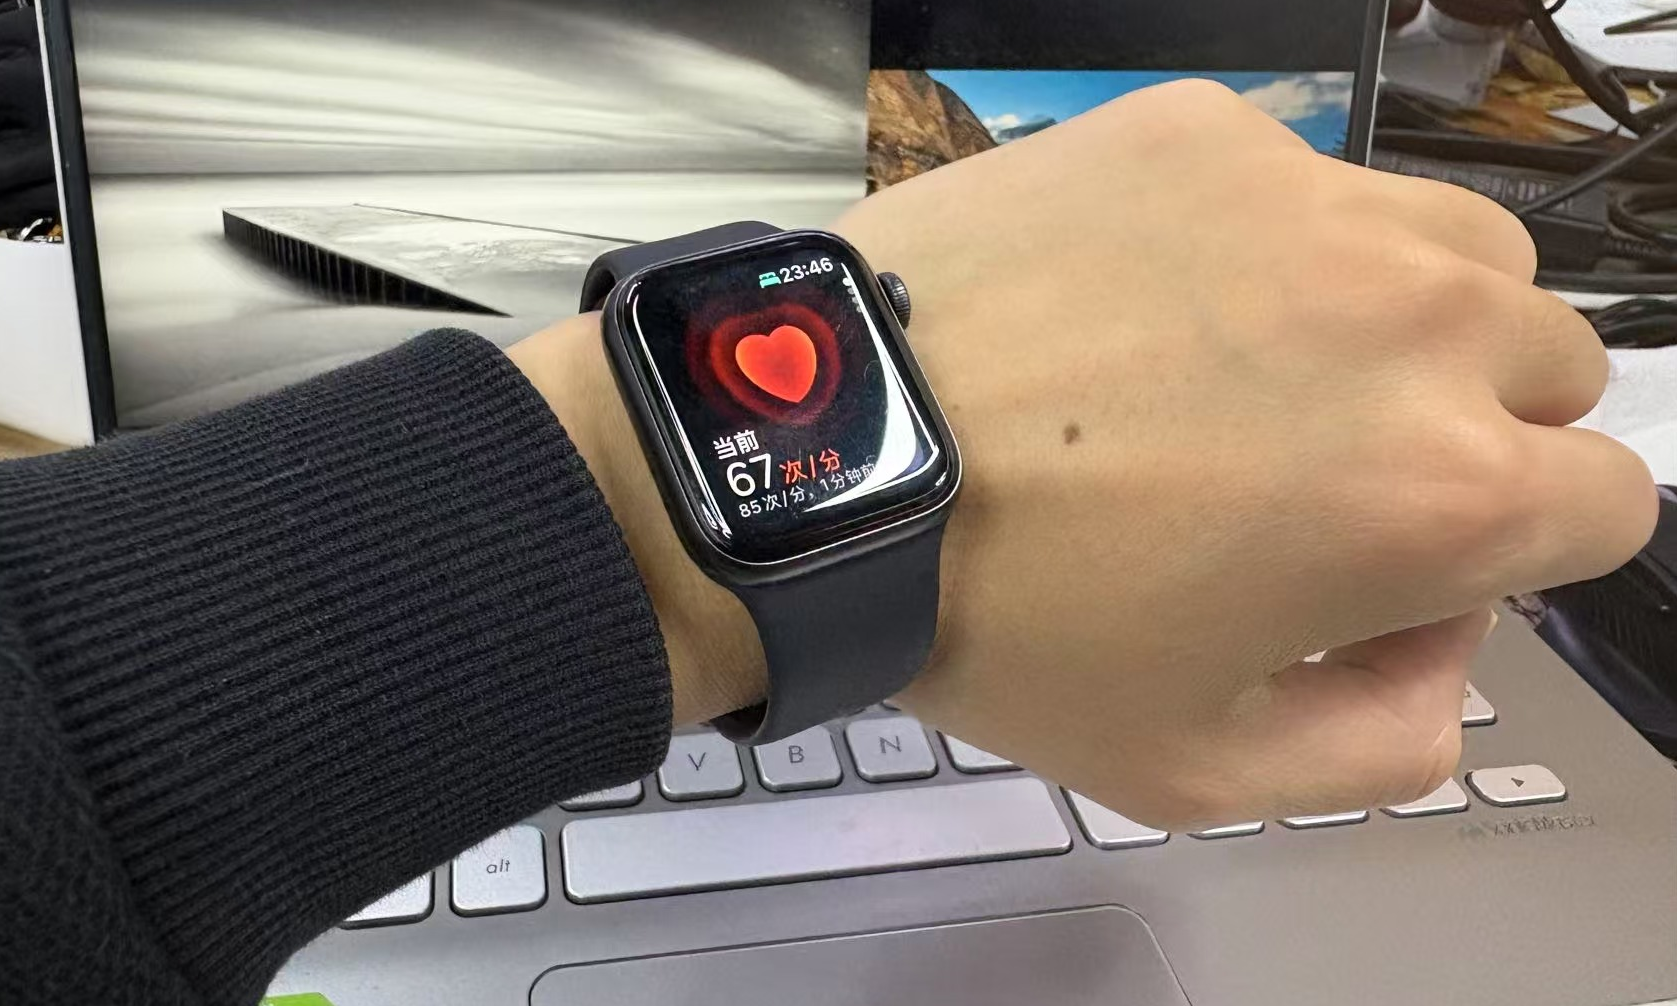
\includegraphics[width=\linewidth]{image/4/apple watch.png}
  \caption{使用Apple Watch实时检测心率}
  \label{fig:apple watch}
\end{figure}

通过分析脑电图和神经影像数据,人工智能系统能够早期检测阿尔茨海默病和帕金森病等神经系统疾病。例如,NVIDIA与多家医疗机构合作,开发了基于深度学习的神经影像分析工具,能够早期识别阿尔茨海默病的生物标志物,支持早期干预和治疗。

\paragraph{个性化预防策略制定}

基于个体的风险评估和疾病预测,人工智能技术能够制定个性化的预防策略,帮助个体降低疾病风险。通过结合基因信息、健康数据和行为模式,人工智能系统能够推荐适合的生活方式调整、饮食计划和运动方案。

人工智能根据个体的基因信息和健康数据,制定个性化的饮食和运动计划。例如,基于个体基因中的代谢相关变异,人工智能系统可以推荐适合的饮食类型和运动强度,以优化体重管理和代谢健康。

此外,通过整合可穿戴设备和人工智能分析,智能健康管理系统能够实时监测个体的健康状况,提供个性化的健康建议。例如,Fitbit和Apple Health等平台利用人工智能技术分析用户的步数、睡眠质量和心率数据,提供个性化的健康指导,支持疾病预防和健康管理。

\subsubsection{3.小结}

个性化医疗与基因分析通过人工智能技术的应用,实现了基于个体基因信息和健康数据的精准医疗服务。计算机视觉和深度学习在基因测序自动化、基因变异检测与注释、基因表达分析以及多组学数据整合中发挥了重要作用,提升了基因数据分析的效率和准确性。同时,人工智能在预测性医疗中的应用,通过风险因素识别、预测模型构建、早期疾病检测和个性化预防策略制定,显著提高了疾病预防和管理的效果。随着人工智能技术的不断发展,个性化医疗与基因分析将在未来医疗实践中发挥更加关键的作用,推动医疗服务向更加精准、高效和个性化的方向发展。

\subsection{远程医疗与虚拟健康助手}

远程医疗与虚拟健康助手是智慧医疗的重要组成部分,通过人工智能技术的应用,实现了医疗服务的智能化、便捷化和个性化。远程医疗服务利用人工智能进行远程诊断、健康监测和远程手术,极大地提升了医疗资源的利用效率和患者的就医体验。虚拟健康助手则通过生成式人工智能技术,提供智能健康咨询与管理,帮助用户进行健康数据分析和健康行为指导。以下将详细探讨人工智能在远程医疗服务和虚拟健康助手中的具体应用及其技术实现。

\subsubsection{1.远程医疗服务}

远程医疗服务利用人工智能技术,通过互联网和5G通信技术,实现远程诊断、健康监测和远程手术,突破了地域和时间的限制,提升了医疗服务的覆盖范围和响应速度。人工智能在远程医疗中的主要应用包括远程诊断支持、智能健康监测系统和机器人辅助手术。

\begin{figure}[ht]
  \centering
  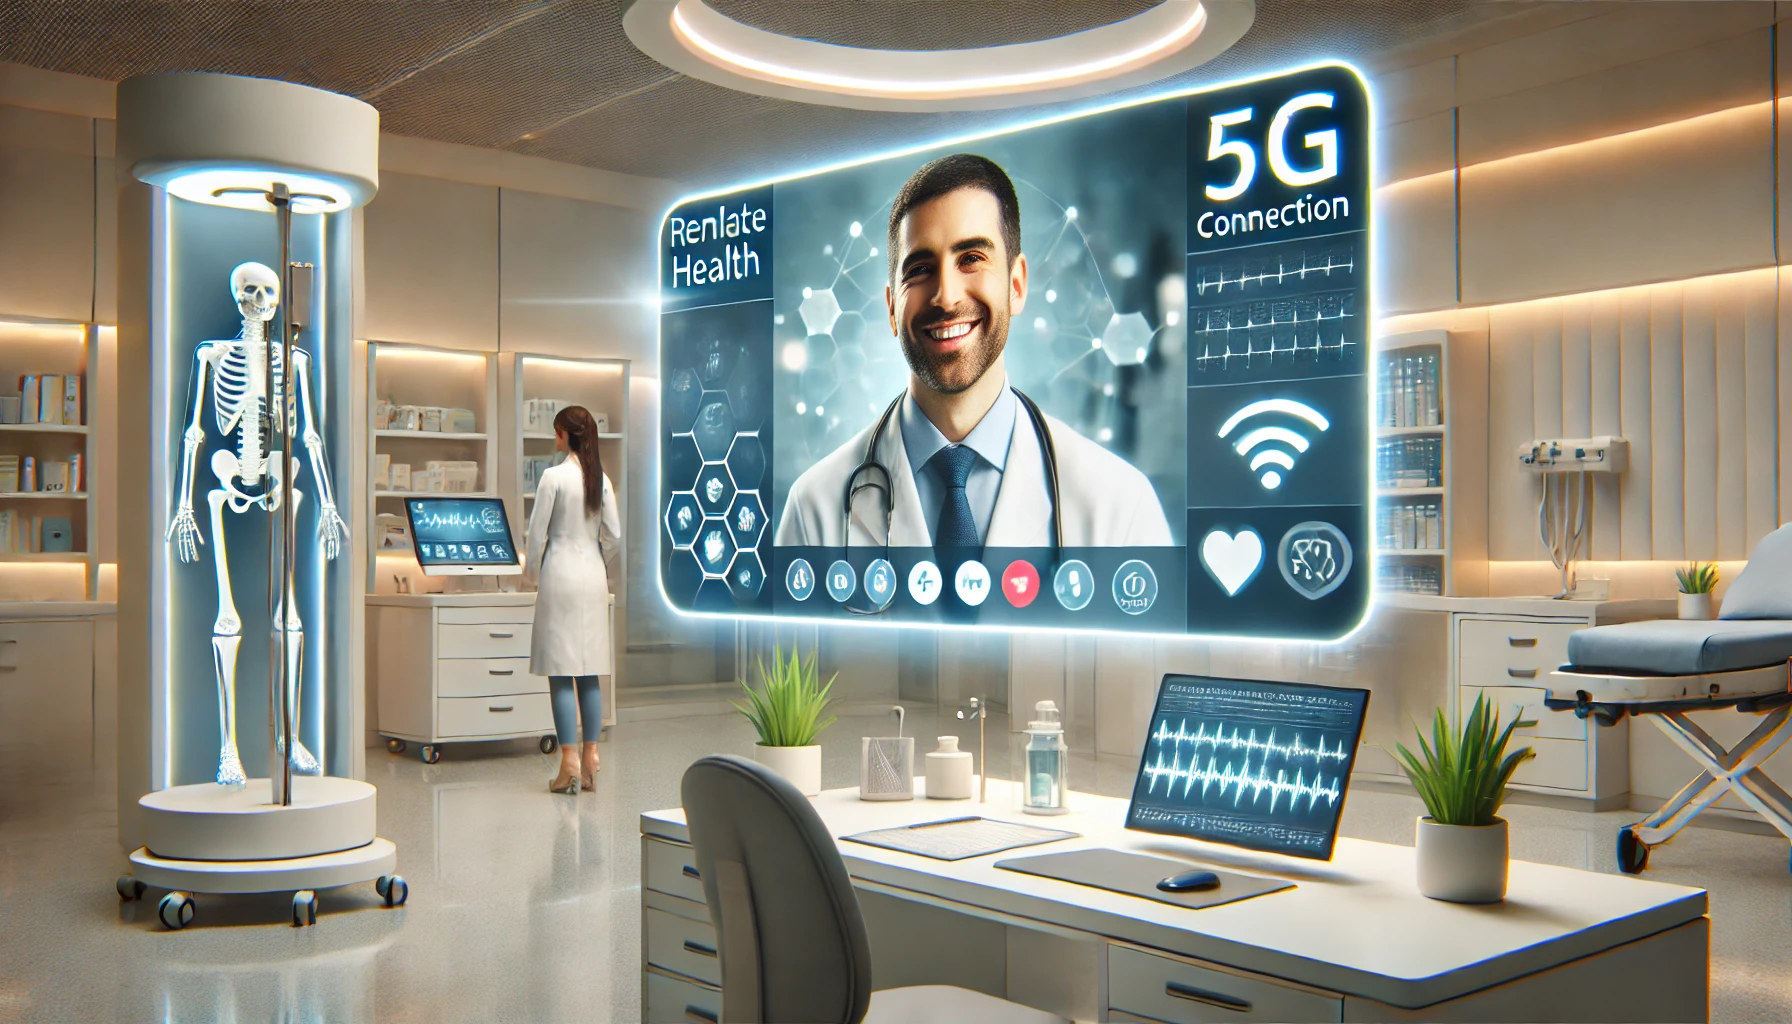
\includegraphics[width=\linewidth]{image/4/远程医疗.png}
  \caption{基于5G通讯的远程医疗服务(图片由AI生成)}
  \label{fig:远程医疗}
\end{figure}

\paragraph{远程诊断支持}

远程诊断支持系统通过人工智能技术,分析患者的症状、病史和医疗影像,辅助医生进行疾病诊断和治疗方案制定。主要技术包括自然语言处理、计算机视觉和深度学习。

具体来说,通过自然语言处理技术,分析患者通过在线平台提交的症状描述,结合深度学习模型,预测可能的疾病类型。

医疗影像远程分析则利用计算机视觉和深度学习技术,人工智能系统能够远程分析患者上传的X光、MRI、CT等医疗影像,自动识别异常病变,提供初步诊断结果。例如,Google的DeepMind开发的人工智能系统能够准确识别眼科疾病,通过远程分析眼底扫描图像,辅助医生进行诊断。

由人工智能驱动的智能问诊系统则能够模拟医生的问诊过程,收集患者的健康信息,提供初步的健康评估和就医建议。例如,Babylon Health的智能问诊应用通过人工智能分析用户的健康信息,提供个性化的医疗建议和预约医生服务。

\paragraph{智能健康监测系统}

智能健康监测系统利用人工智能技术,实时监测和分析患者的生理数据,提供持续的健康管理和疾病预防服务。核心技术包括物联网、机器学习和大数据分析。

具体应用包括健康数据整合与分析,人工智能系统能够整合来自可穿戴设备(如智能手表、健康追踪器)的实时生理数据,如心率、血压、血氧水平等,实时监测患者的健康状态,及时发现异常。例如,Apple Watch结合人工智能算法,能够实时监测用户的心率变化,检测心房颤动等心律失常,及时发出警报。远程健康监控平台则能够整合多源数据,提供全面的健康状况分析和报告。Fitbit Health Solutions利用人工智能技术分析用户的活动数据、睡眠质量和生理指标,提供个性化的健康建议和预防措施。

在慢性病管理中,人工智能通过持续监测患者的健康数据,提供个性化的疾病管理方案,帮助患者控制病情,减少急性发作的风险。例如,Livongo的智能健康管理平台针对糖尿病患者,实时监测血糖水平,提供饮食和运动建议,优化病情管理。

\subsubsection{2.虚拟健康助手}

虚拟健康助手利用生成式人工智能技术,提供智能健康咨询与管理,帮助用户进行健康数据分析和健康行为指导。在这一领域,人工智能的主要应用包括智能健康问答系统、健康数据分析与管理以及个性化健康指导。

\paragraph{智能健康问答系统}

智能健康问答系统通过自然语言处理和生成式人工智能技术,能够理解用户的健康问题,提供准确、及时的健康咨询和建议。

具体而言,人工智能系统能够理解用户的健康问题,通过自然语言生成技术,提供详细的健康信息和建议。例如,虚拟健康助手通过人工智能技术,分析用户的健康问题,提供个性化的健康咨询和初步诊断建议。

此外,人工智能系统还能够引导用户进行疾病自查,通过分析用户的回答,评估其患病风险,并建议是否需要就医。例如,智能健康助手通过互动问答,帮助用户自查症状,评估疾病风险,并推荐相应的医疗服务。

同时,智能虚拟助手能够快速访问和检索庞大的医疗知识库,提供权威的健康信息和最新的医学研究成果。例如,虚拟助手利用人工智能技术,实时检索医疗数据库,为用户提供准确的健康信息和专家级的建议。

\paragraph{健康数据分析与管理}

在健康数据分析与管理方面,人工智能技术整合和分析用户的健康数据,提供全面的健康状态评估和管理方案。

具体应用包括健康数据整合与分析,人工智能系统能够整合来自不同来源的健康数据,如电子健康记录(EHR)、可穿戴设备、基因数据等,进行综合分析,提供全面的健康评估。

疾病预测与风险评估方面,人工智能系统通过分析用户的健康数据,预测潜在的疾病风险,提供早期预警和干预建议,例如某人工智能健康管理平台通过分析用户的健康数据,预测糖尿病和心血管疾病的风险,提供个性化的预防和管理方案。

此外,人工智能系统还能够实时监测用户的健康趋势,生成详细的健康报告,帮助用户了解自身的健康状况和变化。例如,某健康监测系统通过人工智能分析用户的活动数据和生理指标,生成详细的健康趋势报告,支持用户的健康管理和目标设定。

\paragraph{个性化健康指导}

在个性化健康指导方面,人工智能技术结合用户的健康数据和个体差异,提供个性化的健康行为指导和生活方式建议,促进健康行为的养成和维持。

具体应用包括个性化饮食与运动建议,人工智能系统根据用户的健康数据、基因信息和生活习惯,提供个性化的饮食和运动计划。例如,Noom的智能健康指导平台通过分析用户的饮食习惯和活动水平,制定个性化的饮食和运动计划,帮助用户实现减重和健康管理目标。

行为改变与健康激励方面,人工智能系统能够通过行为科学和机器学习算法,设计个性化的健康激励策略,促进用户的健康行为改变,例如某虚拟健康助手通过人工智能技术,提供个性化的健康激励和行为指导,帮助用户养成健康的生活习惯。

心理健康支持方面,智能虚拟助手能够提供心理健康支持,通过情感分析和自然语言生成技术,提供心理咨询和情感支持,帮助用户应对压力和情绪问题。例如,一款智能心理健康助手通过聊天交互,提供认知行为疗法\footnote{认知行为疗法(Cognitive Behavioral Therapy, CBT)是一种重要且广泛应用的心理治疗方法。它的核心理念在于,通过识别和改变个体内心的负面思维模式,帮助人们提升情绪状态和改善行为表现。这种治疗方法强调了思维方式与情感及行动之间的密切关系,使患者能够在认知上调整不健康的模式。}技术,帮助用户管理压力和焦虑情绪。

\subsubsection{3.小结}

远程医疗与虚拟健康助手通过人工智能技术的应用,实现了医疗服务的智能化和个性化,显著提升了医疗资源的利用效率和患者的就医体验。远程医疗服务利用人工智能进行远程诊断、健康监测和远程手术,突破了地域和时间的限制,提升了医疗服务的覆盖范围和响应速度。虚拟健康助手则通过生成式人工智能技术,提供智能健康咨询与管理,帮助用户进行健康数据分析和健康行为指导,促进健康管理的个性化和持续化。随着人工智能技术的不断发展,远程医疗与虚拟健康助手将在未来医疗实践中发挥更加关键的作用,推动医疗服务向更加精准、高效和个性化的方向发展。

\section {总结}

% 本章深入探讨了人工智能在智慧生活、智慧驾驶和智慧医疗三个关键领域的广泛应用及其深远影响。人工智能正不断革新人们的生活方式、出行模式和医疗服务,推动社会向更加智能化、高效化和个性化的方向发展。

% 在智慧生活方面,智能家居通过物联网和人工智能技术实现设备的互联互通与智能管理,显著提升了生活的便利性、安全性和舒适度。智能灯光、智能温控和智能安防系统不仅能够自动调节环境参数,还能通过数据分析优化能源使用和增强家庭安全。同时,智能助理与语音交互技术使人与机器的交流更加自然,诸如Google Assistant、Apple Siri等智能助理能够理解用户意图,提供个性化服务和建议。智能娱乐与个性化推荐通过分析用户行为和偏好,结合深度学习技术,提供量身定制的内容推荐,极大地丰富了用户的娱乐体验。

% 在智慧驾驶领域,自动驾驶技术依托计算机视觉和深度学习,实现了车辆的自主导航和控制,确保行驶的安全性和效率。计算机视觉通过多传感器数据感知环境,识别道路、障碍物和行人,为深度学习决策系统提供精准的数据支持。车联网与智能交通管理通过车联网技术,实现车辆与车辆、车辆与基础设施之间的实时通信,优化交通流量和提升交通安全。人工智能算法在智能交通系统中的应用,能够智能化地管理交通信号灯、优化行驶路线、预防交通事故并提高应急响应效率,推动智慧城市的发展。

% 在智慧医疗方面,人工智能技术通过计算机视觉和深度学习,实现了医疗影像的自动识别与分析,辅助医生进行精准诊断,减少人为误差并提高诊断效率。个性化医疗与基因分析利用人工智能对基因数据进行深度解析,揭示个体基因信息与疾病风险的关联,支持个性化的治疗方案和预防措施。此外,远程医疗与虚拟健康助手通过人工智能技术,实现了远程诊断、健康监测和智能健康管理,突破了地域限制,提升了医疗资源的利用效率,并通过智能问答和个性化健康指导,促进健康管理的持续化和个性化。

% 综上所述,人工智能与物联网技术的深度融合在智慧生活、智慧驾驶和智慧医疗领域带来了巨大变革。智能家居、智能助理和个性化推荐系统提升了日常生活的便利性和个性化体验;自动驾驶和车联网技术推动了交通系统的智能化与安全性;智慧医疗通过精准诊断、个性化治疗和远程医疗服务,显著提升了医疗服务的质量和效率。随着技术的不断进步,人工智能将在更多领域发挥重要作用,推动社会向更加智能化、高效化和个性化的方向发展。

本章深入探讨了人工智能在智慧生活、智慧驾驶和智慧医疗三大领域的广泛应用及其深远影响。智慧生活方面,物联网与人工智能技术使智能家居设备互联互通,提升了生活的便利性、安全性与舒适度,智能助理和个性化推荐进一步丰富了用户体验。智慧驾驶领域,自动驾驶依托计算机视觉和深度学习实现自主导航,车联网技术优化交通流量与安全,推动交通系统智能化。智慧医疗方面,人工智能通过自动识别医疗影像、个性化基因分析及远程医疗服务,提升了诊断的精准性和医疗资源的利用效率。综上,人工智能与物联网的深度融合在这三个关键领域带来了巨大变革,推动社会向更加智能化、高效化和个性化的方向发展,预示着人工智能将在更多领域持续发挥重要作用。

\section*{习题}
\begin{enumerate}
\item \textbf{简述家庭自动化系统中物联网技术与人工智能的结合是如何实现设备的智能管理的?}

参考答案: 家庭自动化系统通过将物联网技术与人工智能相结合,实现了设备的智能管理。物联网技术通过各种传感器和连接设备将家中的各个设备互联,使它们能够相互通信和协作。人工智能则通过分析和处理这些设备收集到的数据,学习用户的习惯和偏好,从而自动优化设备的运行。例如,智能温控系统可以根据用户的日常作息自动调节室内温度;智能灯光系统能够根据环境光线和用户活动自动调节灯光亮度和颜色;智能安防系统则可以实时监控家中的安全状况,自动识别异常情况并采取相应措施。通过这种结合,家庭自动化系统能够实现设备的自主调节和优化,提升生活的便利性和舒适度。

\item \textbf{请你举例你使用过的生成式人工智能工具?}

参考答案: 我使用过的生成式人工智能工具之一是OpenAI的ChatGPT。ChatGPT是一种基于深度学习的自然语言生成模型,能够理解和生成自然语言文本,应用广泛于聊天、内容创作、语言翻译等领域。例如,我可以使用ChatGPT来撰写文章、回答问题、生成代码、提供学习建议等。此外,我还使用过DALL·E,它是一种生成式人工智能模型,可以根据文本描述生成逼真的图像,广泛应用于艺术创作、设计和视觉内容生成中。这些生成式人工智能工具极大地提升了我的工作效率和创作能力,使我能够更快地完成任务和实现创意。

\item \textbf{语音识别技术在智能助理中的作用是什么?其主要工作流程包括哪些步骤?}

参考答案:语音识别技术在智能助理中起着核心作用,通过五个主要步骤将用户的语音指令高效准确地转换为文本或命令,从而实现设备控制和信息获取。首先,麦克风采集用户的语音信号并将其转换为数字信号;其次,对信号进行去噪、回声抑制和增强处理以提高清晰度和识别准确性;然后,从预处理后的信号中提取关键特征。接下来,将这些特征与预先训练的深度神经网络、卷积神经网络或循环神经网络模型进行模式匹配,识别出相应的文字或指令;最后,对识别结果进行语法校正和上下文理解,生成最终的文本输出或执行指令。通过这一系列步骤,语音识别技术有效支撑了智能助理的各种功能,如设备控制、信息查询和任务管理,提升了用户的交互体验。

\item \textbf{协同过滤算法在推荐系统中的作用是什么?请区分基于用户的协同过滤和基于物品的协同过滤。}

参考答案:协同过滤算法是推荐系统的核心,通过分析和预测用户偏好提供个性化内容推荐。主要分为两种类型:基于用户的协同过滤通过计算用户之间的相似度,找到具有相似偏好的用户并推荐他们喜欢的内容,但在用户和物品数量庞大时计算复杂且易受稀疏性和冷启动问题影响;基于物品的协同过滤则通过分析物品之间的相似性,推荐与用户已喜欢的物品相似的其他物品,具有较低的计算复杂度和更高的稳定性,适合处理大规模数据,但对新物品的推荐效果较差。综上所述,协同过滤算法通过用户行为数据提供个性化推荐,基于用户和基于物品的协同过滤各有优缺点,实际应用中常结合使用以提升推荐系统的效果和覆盖率。

\item  \textbf{内容推荐算法如何解决冷启动问题?其主要优势和局限性是什么?}

参考答案:内容推荐算法通过分析物品的内在特征,为用户推荐与其兴趣相似的内容,有效解决了协同过滤中的冷启动问题,即新用户或新物品缺乏足够历史数据导致推荐效果不佳。其解决方式包括分析新物品的内容特征并向感兴趣的用户推荐,以及基于新用户填写的兴趣偏好进行推荐。该算法的主要优势在于不依赖用户的历史行为数据,能够即时为新物品和新用户提供推荐,同时具有较强的解释性,如“因为你喜欢动作片,所以推荐这部新上映的动作片”。然而,内容推荐也存在推荐内容狭窄和依赖内容特征准确性的局限,容易导致推荐内容缺乏多样性,用户难以发现新颖的兴趣点。为了提升推荐效果,通常将内容推荐与协同过滤等其他推荐方法结合使用。

\item \textbf{生成式人工智能如何改变音乐和影视内容的创作与生产方式?请举例说明其影响。}

参考答案:生成式人工智能通过自动生成新数据和内容,显著改变了音乐和影视的创作与生产方式,带来了创新和灵活性,提升了效率并扩展了创作可能性。在音乐创作中,生成式人工智能如OpenAI的Jukedeck和Amper Music能够根据特定风格和情感生成新曲目,降低创作门槛并拓展创意空间,例如AIVA通过学习经典作品创作新的交响乐。在影视制作中,生成式人工智能辅助剧本创作与情节设计,自动生成剧情和对话,提升特效和虚拟角色的生成效率与质量,如GAN技术减少手工制作时间和成本,同时人工智能还能根据剧情生成配乐与音效,增强观影体验,并创建沉浸式的虚拟现实和增强现实内容。具体实例包括OpenAI的Sora能够根据文字描述生成连贯视频,简化制作流程,Amper Music则通过人工智能生成符合需求的背景音乐,降低创作成本。总体而言,生成式人工智能通过自动化创作、多样化创新和提升制作效率,深刻推动了音乐和影视产业的变革与发展,带来了巨大的行业机遇。

\item \textbf{车联网技术中的V2V、V2I和V2P通信模式分别有哪些功能?它们如何提升交通安全和效率?}

参考答案:V2V、V2I和V2P通信模式通过实时信息共享和协作,显著提升了交通系统的安全性和效率。V2V(车辆间通信)通过共享速度、位置和运动信息,实现协同驾驶和碰撞预警,减少事故发生并优化交通流。V2I(车辆与基础设施通信)通过与交通信号灯和道路传感器的实时通信,优化信号控制和行驶路线,缓解交通拥堵并提升道路通行效率,同时支持应急管理。在V2P(车辆与行人通信)中,行人通过智能设备共享位置信息,车辆自动调整行驶行为以避免碰撞,并通过提示系统提醒驾驶员注意行人,从而保障行人安全并保持交通流畅。这些通信模式的综合应用推动了智能交通系统的发展,促进了智慧城市建设,提高了整体交通管理水平。

\item \textbf{简述SAE分级以及每一级的特征}

SAE分级标准由美国汽车工程师协会(SAE)制定,用于划分自动驾驶技术的发展阶段,从0级到5级,总共六个等级。这个分级标准的核心依据是自动驾驶系统中人类驾驶员的介入程度,以帮助评估自动驾驶技术的成熟度和实际应用能力。在0级(无自动化)下,完全由人类驾驶员控制,车辆没有任何自动化功能,驾驶员需要全程控制车辆,包括加速、刹车、转向等所有操作。而在1级(驾驶辅助)中,提供某些辅助功能,如自适应巡航控制或车道保持,但驾驶员必须始终保持控制,并随时接管。当达到2级(部分自动化)时,车辆能够执行多个自动化任务,比如自适应巡航和车道保持系统同时工作,尽管如此,驾驶员仍需保持注意力,并在系统要求时立即接管控制。

进入3级(有条件自动化),车辆能够在特定条件下完成所有驾驶任务,此时驾驶员可以将注意力转向其他活动。然而,在某些情况下,例如在高速公路上,驾驶员需要在系统请求时迅速介入。4级(高度自动化)表示车辆可以在特定环境或条件下完成所有驾驶任务,驾驶员无需参与控制。这一等级的自动驾驶系统能够在如城市道路或特定地理区域内全权负责驾驶,即使驾驶员没有准备好介入。最后,达到5级(完全自动化)是最高等级,车辆能够在任何环境和情况下独立完成所有驾驶任务,无需驾驶员干预。无论是城市街道还是高速公路,车辆都能自我驾驶,完全实现无人驾驶。总体而言,随着等级的提升,自动驾驶系统的能力不断增强,人类驾驶员的介入需求逐渐减少,最终达到完全自动化的无人驾驶。

\item \textbf{计算机视觉技术如何提升医疗影像分析的准确性和效率?请举例说明。}

参考答案:计算机视觉技术通过模拟人类视觉系统,自动分析和解读医疗影像数据,显著提升了影像分析的准确性和效率。在准确性方面,计算机视觉通过深度学习模型自动识别病变区域,如肿瘤和结节,精确分割并测量其大小和形状,确保分析结果的一致性和标准化。在效率方面,人工智能能够快速处理大量影像数据,自动生成分析报告,并实现实时监控与诊断支持。例如,使用卷积神经网络分析乳腺X光影像自动检测早期乳腺癌,Google DeepMind的人工智能系统准确识别肺部结节,提高肺癌早期发现率,以及通过分析MRI影像自动检测阿尔茨海默病和帕金森病的早期标志物。总体而言,计算机视觉技术不仅帮助医生更快速、准确地诊断疾病,减少工作负担,还提升了医疗服务的整体质量和效率,随着技术的不断进步,计算机视觉将在医疗影像分析中发挥越来越重要的作用,推动医疗行业的智能化发展。

\item \textbf{请你举例生活中的虚拟健康助手。}

% 生活中有许多虚拟健康助手应用,它们利用人工智能技术为用户提供健康监测、咨询和管理服务。例如,Apple Health 是苹果公司推出的一款健康管理应用,通过iPhone和Apple Watch等设备收集用户的健康数据,帮助用户跟踪每日步数、运动量、心率和睡眠质量等信息。此外,Apple Health还能与第三方应用集成,为用户提供个性化的健康建议。类似的,Google Fit 也是一款健康管理应用,专为Android设备和可穿戴设备设计,通过收集运动数据帮助用户设定健康目标,并与其他健康设备兼容,提供步数、运动时长、卡路里消耗等信息。

% 另外,Amazon Halo 结合人工智能技术的健康监测设备,通过腕带收集用户的身体数据,如运动、睡眠、体重和体脂等,并且内置情绪分析功能,分析用户的声音来评估情绪状态,进一步提供个性化健康指导。Babylon Health 则是一款虚拟健康助手应用,用户可以通过手机与AI医生进行对话,接受初步健康评估,甚至获得诊断建议,同时还可以连接到真实医生进行视频诊疗。对于女性用户来说,Flo 是一款帮助女性追踪月经周期、排卵期等生理过程的应用,利用人工智能提供个性化的健康建议,包括饮食、锻炼和心理健康方面的指导。

% 总体而言,这些虚拟健康助手通过收集并分析用户的健康数据,结合智能算法提供个性化的健康建议,未来随着技术的不断进步,它们将在健康管理中扮演越来越重要的角色。

许多虚拟健康助手应用在人们的生活中发挥着重要作用。它们使用人工智能技术为用户提供健康监测、咨询和管理服务。以Apple Health为例,这是苹果公司推出的一款健康管理应用。通过iPhone和Apple Watch等设备,Apple Health收集用户的健康数据。这个应用帮助用户跟踪每日步数、运动量、心率和睡眠质量。此外,Apple Health还能与第三方应用集成,提供个性化的健康建议。

另一款类似的应用是Google Fit。它专为Android设备和可穿戴设备设计。Google Fit通过收集运动数据帮助用户设定健康目标。该应用兼容其他健康设备,提供步数、运动时长和卡路里消耗等信息。

总体而言,这些虚拟健康助手通过收集和分析用户的健康数据,利用智能算法提供个性化建议。随着技术的不断进步,它们在健康管理中的地位将愈加重要。

\end{enumerate}